\documentclass[conference]{IEEEtran}
\usepackage{graphicx}
\usepackage{booktabs}
\usepackage{amsmath}
\usepackage{amssymb}
\usepackage{subcaption}
\usepackage{multirow}
\usepackage{xcolor}
\graphicspath{{figures/}}

\begin{document}

\title{Temporal Multiplexing via Trainable Synaptic Delays\\ in Spiking Neural Networks}

\author{\IEEEauthorblockN{Draft for internal review}
\IEEEauthorblockA{Working paper -- not for distribution\\
Generated from experiment logs \texttt{EXPERIMENT\_LOG.md}, \texttt{EXPERIMENT\_TABLE.md}, \texttt{CLAUDE.md}}}

\maketitle

\begin{abstract}
We ask whether trainable synaptic delays let a spiking neural network (SNN) with a
\emph{fixed} number of hidden neurons and a fixed energy (spike) budget answer more
independent boolean queries per trial than a delay-free baseline -- i.e., whether delays
enable genuine \emph{temporal multiplexing} rather than merely improving single-task
accuracy. Using a minimal two-input boolean-logic testbed and leaky integrate-and-fire
(LIF) neurons, we progressively tighten three experimental designs (serial slots,
synchronous multi-channel, and shared-channel sequential injection) to separate three
distinct contributions of delays: \emph{temporal alignment}, \emph{adaptive routing
capacity}, and \emph{decoder-limited multiplexing}. We show that delays are
structurally necessary for shared-channel multiplexing (weight-only networks plateau at
chance-adjacent accuracy regardless of decoder), that alignment dominates capacity by a
factor of $\sim$4, and that a nonlinear readout raises the achievable load from
\emph{Max K@90\%=2} to \emph{Max K@90\%=3} on top of a fixed 50-neuron budget. A causal
$2\times2$ ablation rules out the confound that the nonlinear readout alone is
responsible. We then show the same mechanism, and the same capacity ceiling, generalises
to mixed-operation trials once data volume and hidden-layer capacity are matched to the
single-operation case. We close with a literature-grounded discussion of why a ceiling
near $K{=}3$ is a plausible order of magnitude, and a set of concretely scoped open
experiments (untested input/output topologies, energy-matched comparisons, a non-SNN
baseline, and a theoretical account of the linear-vs-nonlinear decodability gap) that
would be needed before this work is conference-submission-ready.
\end{abstract}

\section{Introduction}

Biological synapses and axons impose delays that vary by orders of magnitude depending
on conduction distance and myelination, and a long line of neuroscience work has argued
that this temporal structure is not incidental noise but a computational resource:
oscillatory phase coding lets a population of neurons multiplex several discrete items
within one cycle \cite{lisman1995storage,cowan2001magical}, and delay-structured spike
timing can index combinatorially many ``polychronous'' assemblies in a fixed-size network
\cite{izhikevich2006polychronization}. Communication between cortical areas has likewise
been argued to depend on the relative timing/phase of oscillations rather than only on
firing rate \cite{fries2005mechanism,buzsaki2010neural}.

In machine-learning-oriented SNN research, by contrast, trainable delays are almost
always evaluated purely as an accuracy or efficiency lever on a fixed task -- e.g.\ on
spoken-word or vision benchmarks \cite{hammouamri2024learning,sun2022axonal,%
sun2023adaptive,patino2024colearning} -- not as a mechanism that changes \emph{how much
work} a fixed-size network can do. This leaves a specific question understudied:

\begin{quote}
\emph{Given a fixed hidden-layer size $h$ and a fixed energy budget (spikes per trial),
can trainable synaptic delays let an SNN answer more independent queries $K$ per trial
than a weight-only network, at matched accuracy?}
\end{quote}

We study this question on a deliberately minimal testbed -- two-input boolean logic
operations with rate-coded inputs and LIF neurons -- precisely because it gives exact
ground truth and lets us isolate \emph{mechanism} rather than fight dataset complexity.
Our primary metric throughout is \textbf{Max K@$\tau$}: the largest number of
simultaneously-processed queries $K$ for which trial accuracy stays $\geq\tau$ under a
fixed hidden-neuron budget. We compare three training regimes: \texttt{weights\_only}
(delays fixed at 0), \texttt{delays\_only} (weights frozen after initialisation), and
\texttt{weights\_and\_delays} (both trained).

\textbf{Contributions.}
\begin{itemize}
\item A progressive three-design protocol (serial-readout $\to$ dedicated-channel $\to$
shared-channel, abbreviated SR/DC/SC below; Section
\ref{sec:step2}) that decomposes the benefit of delays into \emph{alignment} and
\emph{capacity} components, and isolates a design (the SC design) in which weights are
\emph{structurally} incapable of solving the task without delays.
\item A causal $2\times2$ ablation (readout type $\times$ delay configuration, Section
\ref{sec:ablation}) showing the capacity gain is attributable to delay-structured
representations, not to the nonlinear readout alone.
\item A capacity-scaling study (neuron-count sweep, Section \ref{sec:ablation}) showing
the $K{=}2\to3$ ceiling is decoder-, not neuron-count-, limited.
\item A generalisation study (Section \ref{sec:step3}) showing the same mechanism and the
same capacity ceiling reproduce on mixed-operation trials once data volume and capacity
are matched to the single-operation case.
\item A literature-grounded discussion (Section \ref{sec:discussion}) of why
Max K@90\%=3 is a plausible biological/computational order of magnitude, and a fully
scoped Future Work section (Section \ref{sec:future}) listing exactly which experiments
remain to make this submission-ready.
\end{itemize}

\section{Related Work}

\textbf{Training SNNs with gradients.} Discrete spiking nonlinearities are non-differentiable,
so practical SNN training relies on surrogate gradients
\cite{neftci2019surrogate}, temporal credit-assignment schemes such as SLAYER
\cite{shrestha2018slayer}, or biologically-motivated eligibility-trace methods such as
e-prop \cite{bellec2020solution}. SLAYER defines a probability-density-function-based
spike ``escape rate'' surrogate and additionally backpropagates error through the
synaptic temporal kernel itself, rather than only through a per-timestep membrane
derivative; e-prop replaces backpropagation-through-time (BPTT) with a forward-running,
purely local \emph{eligibility trace} per synapse combined with a top-down learning
signal, avoiding the biologically-implausible backward-in-time pass and the need to store
a full trial's activations that BPTT requires. We use neither: our trials are short
($T\leq55$ steps) and our networks shallow (one or two layers), so there is no long-sequence
memory pressure or biological-plausibility requirement that would justify either method's
added complexity over plain surrogate-gradient BPTT, in the spirit of
\cite{neftci2019surrogate}.

\textbf{Learnable delays.} The most directly comparable recent work treats synaptic or
axonal delay as a first-class trainable parameter alongside weights. Hammouamri et
al.\ \cite{hammouamri2024learning} parameterise delays via dilated convolutions with
learnable spacings (DCLS) and show accuracy gains on standard SNN benchmarks. Sun et
al.\ \cite{sun2022axonal,sun2023adaptive} learn axonal delays as a short-term-memory
mechanism for spoken-word recognition. Pati\~no-Saucedo et al.\ \cite{patino2024colearning}
co-train delays, weights, and adaptation. All of these works report that learnable delays
improve accuracy or efficiency on a \emph{fixed} task; none of them ask whether delays
change the number of independent tasks a fixed-size network can handle \emph{at once}.
That is the gap we address: we hold network size and task difficulty fixed and vary the
number of simultaneous queries $K$, using delay-vs-no-delay as the controlled variable.

\textbf{Temporal multiplexing in neuroscience.} Our framing of $K$ as ``items
multiplexed per cycle'' follows the theta--gamma working-memory literature
\cite{lisman1995storage,cowan2001magical} -- in which a slow ($\theta$, 4--8\,Hz)
oscillation is divided into faster ($\gamma$, 30--80\,Hz) sub-cycles, and a population of
cortical neurons is argued to carry one discrete memory item per sub-cycle, i.e.\ a
phase-multiplexing code -- and the polychronous-group account of delay-based
combinatorial coding \cite{izhikevich2006polychronization}, where fixed axonal delays
cause spikes from different neurons, fired at different times, to arrive at a shared
downstream target simultaneously, producing a reproducible spike chain without requiring
any synchronous firing. We return to these as a quantitative point of comparison in
Section \ref{sec:discussion}.

\section{Methods}

\subsection{Neuron and synapse model}
All experiments use leaky integrate-and-fire (LIF) neurons with a refractory period,
simulated at $dt{=}1\,\mathrm{ms}$. The membrane potential updates as
\begin{equation}
V_i[t] = \lambda V_i[t-1] + (1-\lambda)\,I_i^{syn}[t]\cdot\mathbb{1}[\text{ref}_i[t]\leq0],
\quad \lambda = e^{-dt/\tau_m},
\label{eq:lif}
\end{equation}
with a spike $s_i[t]=\mathbb{1}[V_i[t]-V_{th}\geq0]$ whenever the membrane crosses
threshold, after which $V_i$ resets to $V_{reset}$ and the neuron enters refractory for
$n_{ref}$ steps. Because $s_i[t]$ is non-differentiable, the backward pass uses a
fast-sigmoid surrogate gradient,
\begin{equation}
\frac{\partial s_i[t]}{\partial V_i[t]} \approx \frac{\beta}{(1+\beta|V_i[t]-V_{th}|)^2},
\label{eq:surrogate}
\end{equation}
with steepness $\beta{=}4$.

Discrete synaptic delays $d_{ij}\in[0,d_{\max}]$ are parameterised by a sigmoid mapping
into the valid range,
\begin{equation}
d_{ij} = d_{\max}\cdot\sigma(\theta_{ij}),
\label{eq:delayparam}
\end{equation}
trained by gradient descent jointly with (or independently of, depending on training
mode) the weights $w_{ij}$, using separate learning rates $lr_w$, $lr_d$. The delayed
synaptic current is read out by linearly interpolating between the floor and ceiling of
the (continuous) delay,
\begin{equation}
I_j^{syn}[t] = \sum_i w_{ij}\Big[(1-\alpha_{ij})\,s_i[t{-}\lfloor d_{ij}\rfloor]
+ \alpha_{ij}\,s_i[t{-}\lceil d_{ij}\rceil]\Big],
\label{eq:delayread}
\end{equation}
with $\alpha_{ij}=d_{ij}-\lfloor d_{ij}\rfloor$ -- this interpolation is what gives a
continuous delay a smooth gradient, rather than blocking it at a discrete buffer index.

Our parameter choices ($\tau_m{=}10\,\mathrm{ms}$, $V_{th}{=}1.0$, $dt{=}1\,\mathrm{ms}$,
$n_{ref}{=}2\,\mathrm{ms}$) sit inside the range used elsewhere in the surrogate-gradient
SNN literature: Neftci et al.\ \cite{neftci2019surrogate} report $\tau_m\in[5,20]\,\mathrm{ms}$
as a typical range; Bellec et al.\ \cite{bellec2020solution} use $\tau_m{=}20\,\mathrm{ms}$
for standard (non-adaptive) LIF units in e-prop; Fang et al.\ \cite{fang2021plif}'s
learnable-$\tau_m$ networks converge to values across roughly the same 2--20\,ms range.
We did not tune $\tau_m$ or $V_{th}$ for this task -- they are literature-typical
defaults, not task-fit hyperparameters -- but Section~\ref{sec:ablation}'s
timing-parameter ablation tests this choice directly: raising $\tau_m$ from 10 to
20\,ms \emph{lowers} Max K@90\% to 0 by weakening the sub-window isolation the SR and SC
designs rely on, so the inherited default also happens to be the locally task-optimal
point, not merely an unexamined convention.

\subsection{Training modes}
Three training modes are compared throughout: \texttt{weights\_only} (delays fixed at 0
or a constant $d_0$), \texttt{delays\_only} (weights frozen after random initialisation),
and \texttt{weights\_and\_delays} (both trained). Unless noted, ``$d{=}0$'' refers to
\texttt{weights\_only} with delays fixed at 0, used as the no-delay control.

\subsection{Task and encoding}
The task is two-input boolean logic (AND, OR, NAND, NOR, XOR, XNOR, and the two
implications) with inputs $(A,B)\in\{0,1\}^2$. Inputs are rate-coded: each timestep, a
Bernoulli spike is drawn independently per channel with
\begin{equation}
p_{\text{on/off}} = r_{\text{on/off}}\cdot dt / 1000, \qquad s[t]\sim\mathrm{Bernoulli}(p),
\label{eq:ratecode}
\end{equation}
using $r_{\text{on}}\approx400\,\mathrm{Hz}$ when the corresponding input bit is 1 and
$r_{\text{off}}\approx10\,\mathrm{Hz}$ when it is 0. We rate-code rather than inject
$(A,B)$ as analog 0/1 values directly because an LIF neuron has no channel for a
single-timestep real-valued input -- its only vocabulary is binary spike/no-spike events,
so any quantity must be represented as a temporally-extended pattern of such events, which
Eq.~\eqref{eq:ratecode} provides and Eq.~\eqref{eq:lif}'s leaky integration is designed to
read out. More specific to this paper: our central question is whether \emph{spike
arrival timing} can be routed by delays, so the input itself must carry genuine
spike-timing structure for a delay to act on -- a constant analog current has no timing
structure to delay, which would make the temporal-multiplexing mechanism under study
inapplicable by construction.

Output is decoded as spike count or mean membrane potential over the readout window,
$z=\mathrm{readout}(h)$, trained with
\begin{equation}
\mathcal{L} = -\tfrac{1}{N}\textstyle\sum_n\big[y_n\log\sigma(z_n)
+ (1{-}y_n)\log(1-\sigma(z_n))\big],
\label{eq:loss}
\end{equation}
i.e.\ \texttt{BCEWithLogitsLoss}. Each query is an independent binary decision, so this is
the standard maximum-likelihood loss for Bernoulli-distributed labels given a raw logit
$z$; computing it directly from $z$ (rather than via a separate sigmoid followed by BCE)
is numerically stable for large $|z|$ and gives well-behaved gradients near
confidently-wrong predictions. Eq.~\eqref{eq:loss} does not care whether $z$ is a spike
count, a membrane potential, or an MLP output, so the readout variants compared in
Sections~\ref{sec:pland}--\ref{sec:ablation} (linear, MLP, and the fully-spiking output
layer of Section~\ref{sec:future}) are directly loss-comparable; Sections~\ref{sec:pland}
and~\ref{sec:ablation} discuss the accuracy/interpretability/trainability trade-offs
between them.

\subsection{Evaluation metrics}
\textbf{Max K@$\tau$} -- the largest $K$ at which trial accuracy $\geq\tau$ under fixed
$h$. This follows the same ``capacity at a fixed error tolerance'' convention used to
define storage capacity in associative-memory networks -- the largest pattern count
recallable below a retrieval-error threshold \cite{hopfield1982neural,amit1985storing},
which we revisit quantitatively in Section~\ref{sec:discussion}. There is no universally
correct value of $\tau$ (much as a 95\% confidence level in statistics is a convention,
not a derived quantity), so we report results at both $\tau{=}90\%$ and $\tau{=}95\%$
throughout and confirm our qualitative conclusions hold at either threshold.
\textbf{Energy-normalised throughput} $K/\text{spikes}$ -- queries answered per
hidden spike emitted. \textbf{Latency} -- time from input-window end to readout decision.

\subsection{Three multi-query trial designs}
Table \ref{tab:designs} summarises the three progressively-constrained experimental
designs used in Section \ref{sec:step2}; Fig.~\ref{fig:designschematic} shows their
trial structure schematically, and Fig.~\ref{fig:method} shows the trial structure
of the most constrained one (the SC design) directly, with per-query sub-windows and the shared
readout window visible in the raster.

\begin{table}[t]
\centering
\caption{Three multi-query trial designs (Section \ref{sec:step2}).}
\label{tab:designs}
\begin{tabular}{lccc}
\toprule
Design & Input ch.\ & Readout & Tests \\
\midrule
SR (serial) & 2 (shared) & $K$ windows & alignment vs.\ multiplexing \\
DC (sync.) & $2K$ (dedicated) & 1 (shared) & alignment vs.\ capacity \\
SC (sequential) & 2 (shared) & 1 (shared) & \textbf{pure temporal routing} \\
\bottomrule
\end{tabular}
\end{table}

\begin{figure}[t]
\centering
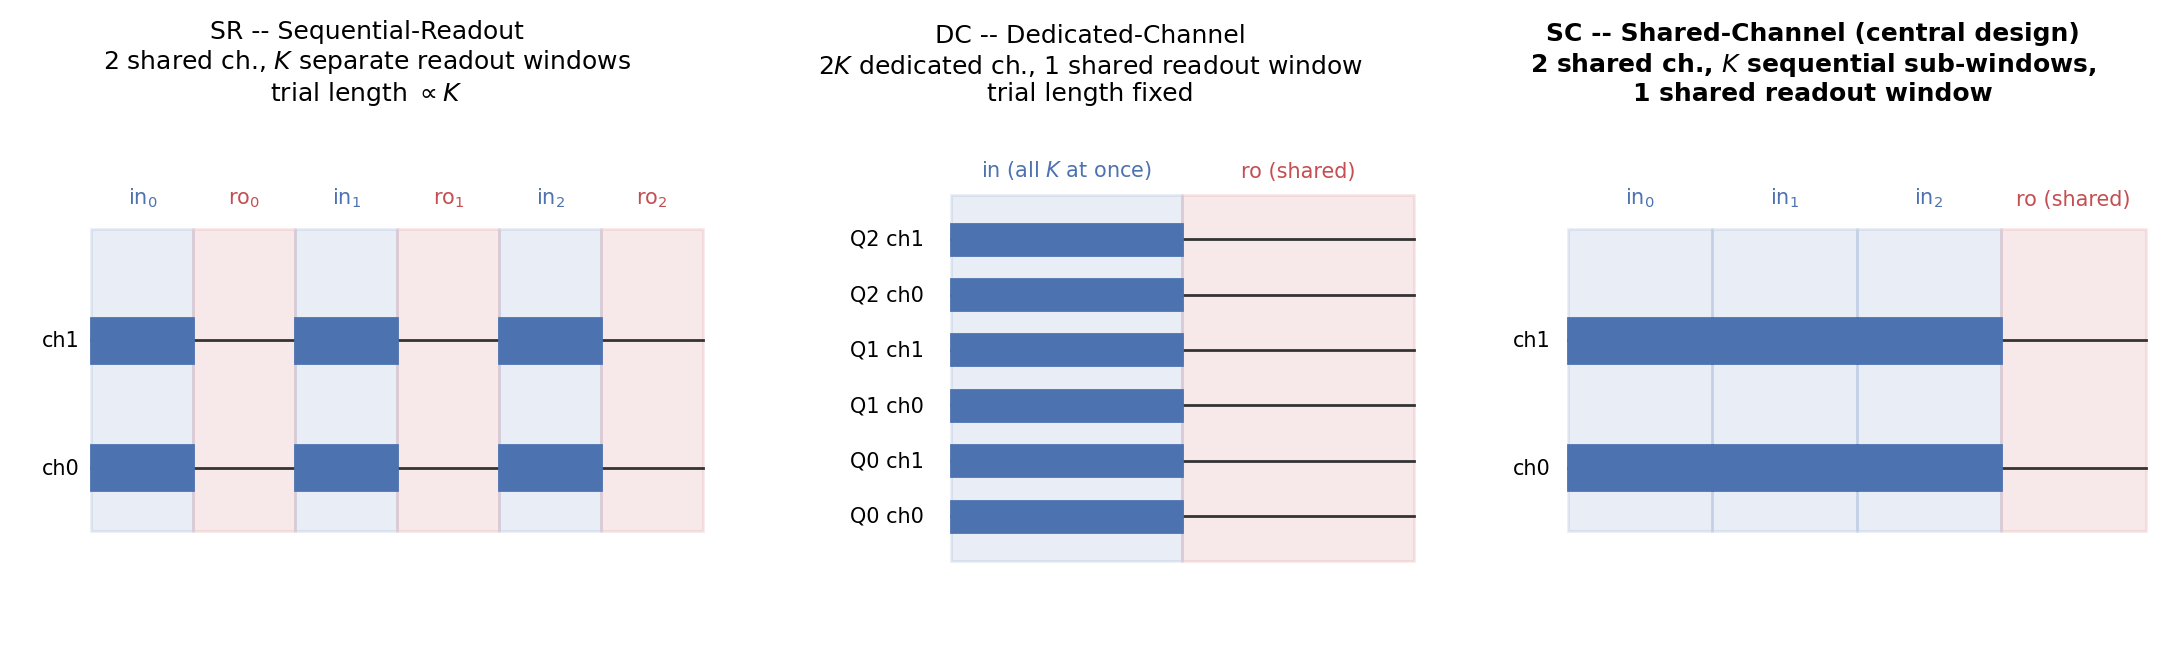
\includegraphics[width=\columnwidth]{fig_design_schematics.png}
\caption{Schematic trial structure of the three designs ($K{=}3$ shown). SR: $K$
independent (input, readout) blocks on 2 shared channels, trial length $\propto K$. DC:
$2K$ dedicated channel pairs fire simultaneously in one fixed-length input window,
followed by one shared readout window. SC: the same 2 channels are reused sequentially
across $K$ input sub-windows, followed by one shared readout window -- the only design in
which weights alone cannot distinguish which query a given input spike belongs to.}
\label{fig:designschematic}
\end{figure}

\begin{figure}[t]
\centering
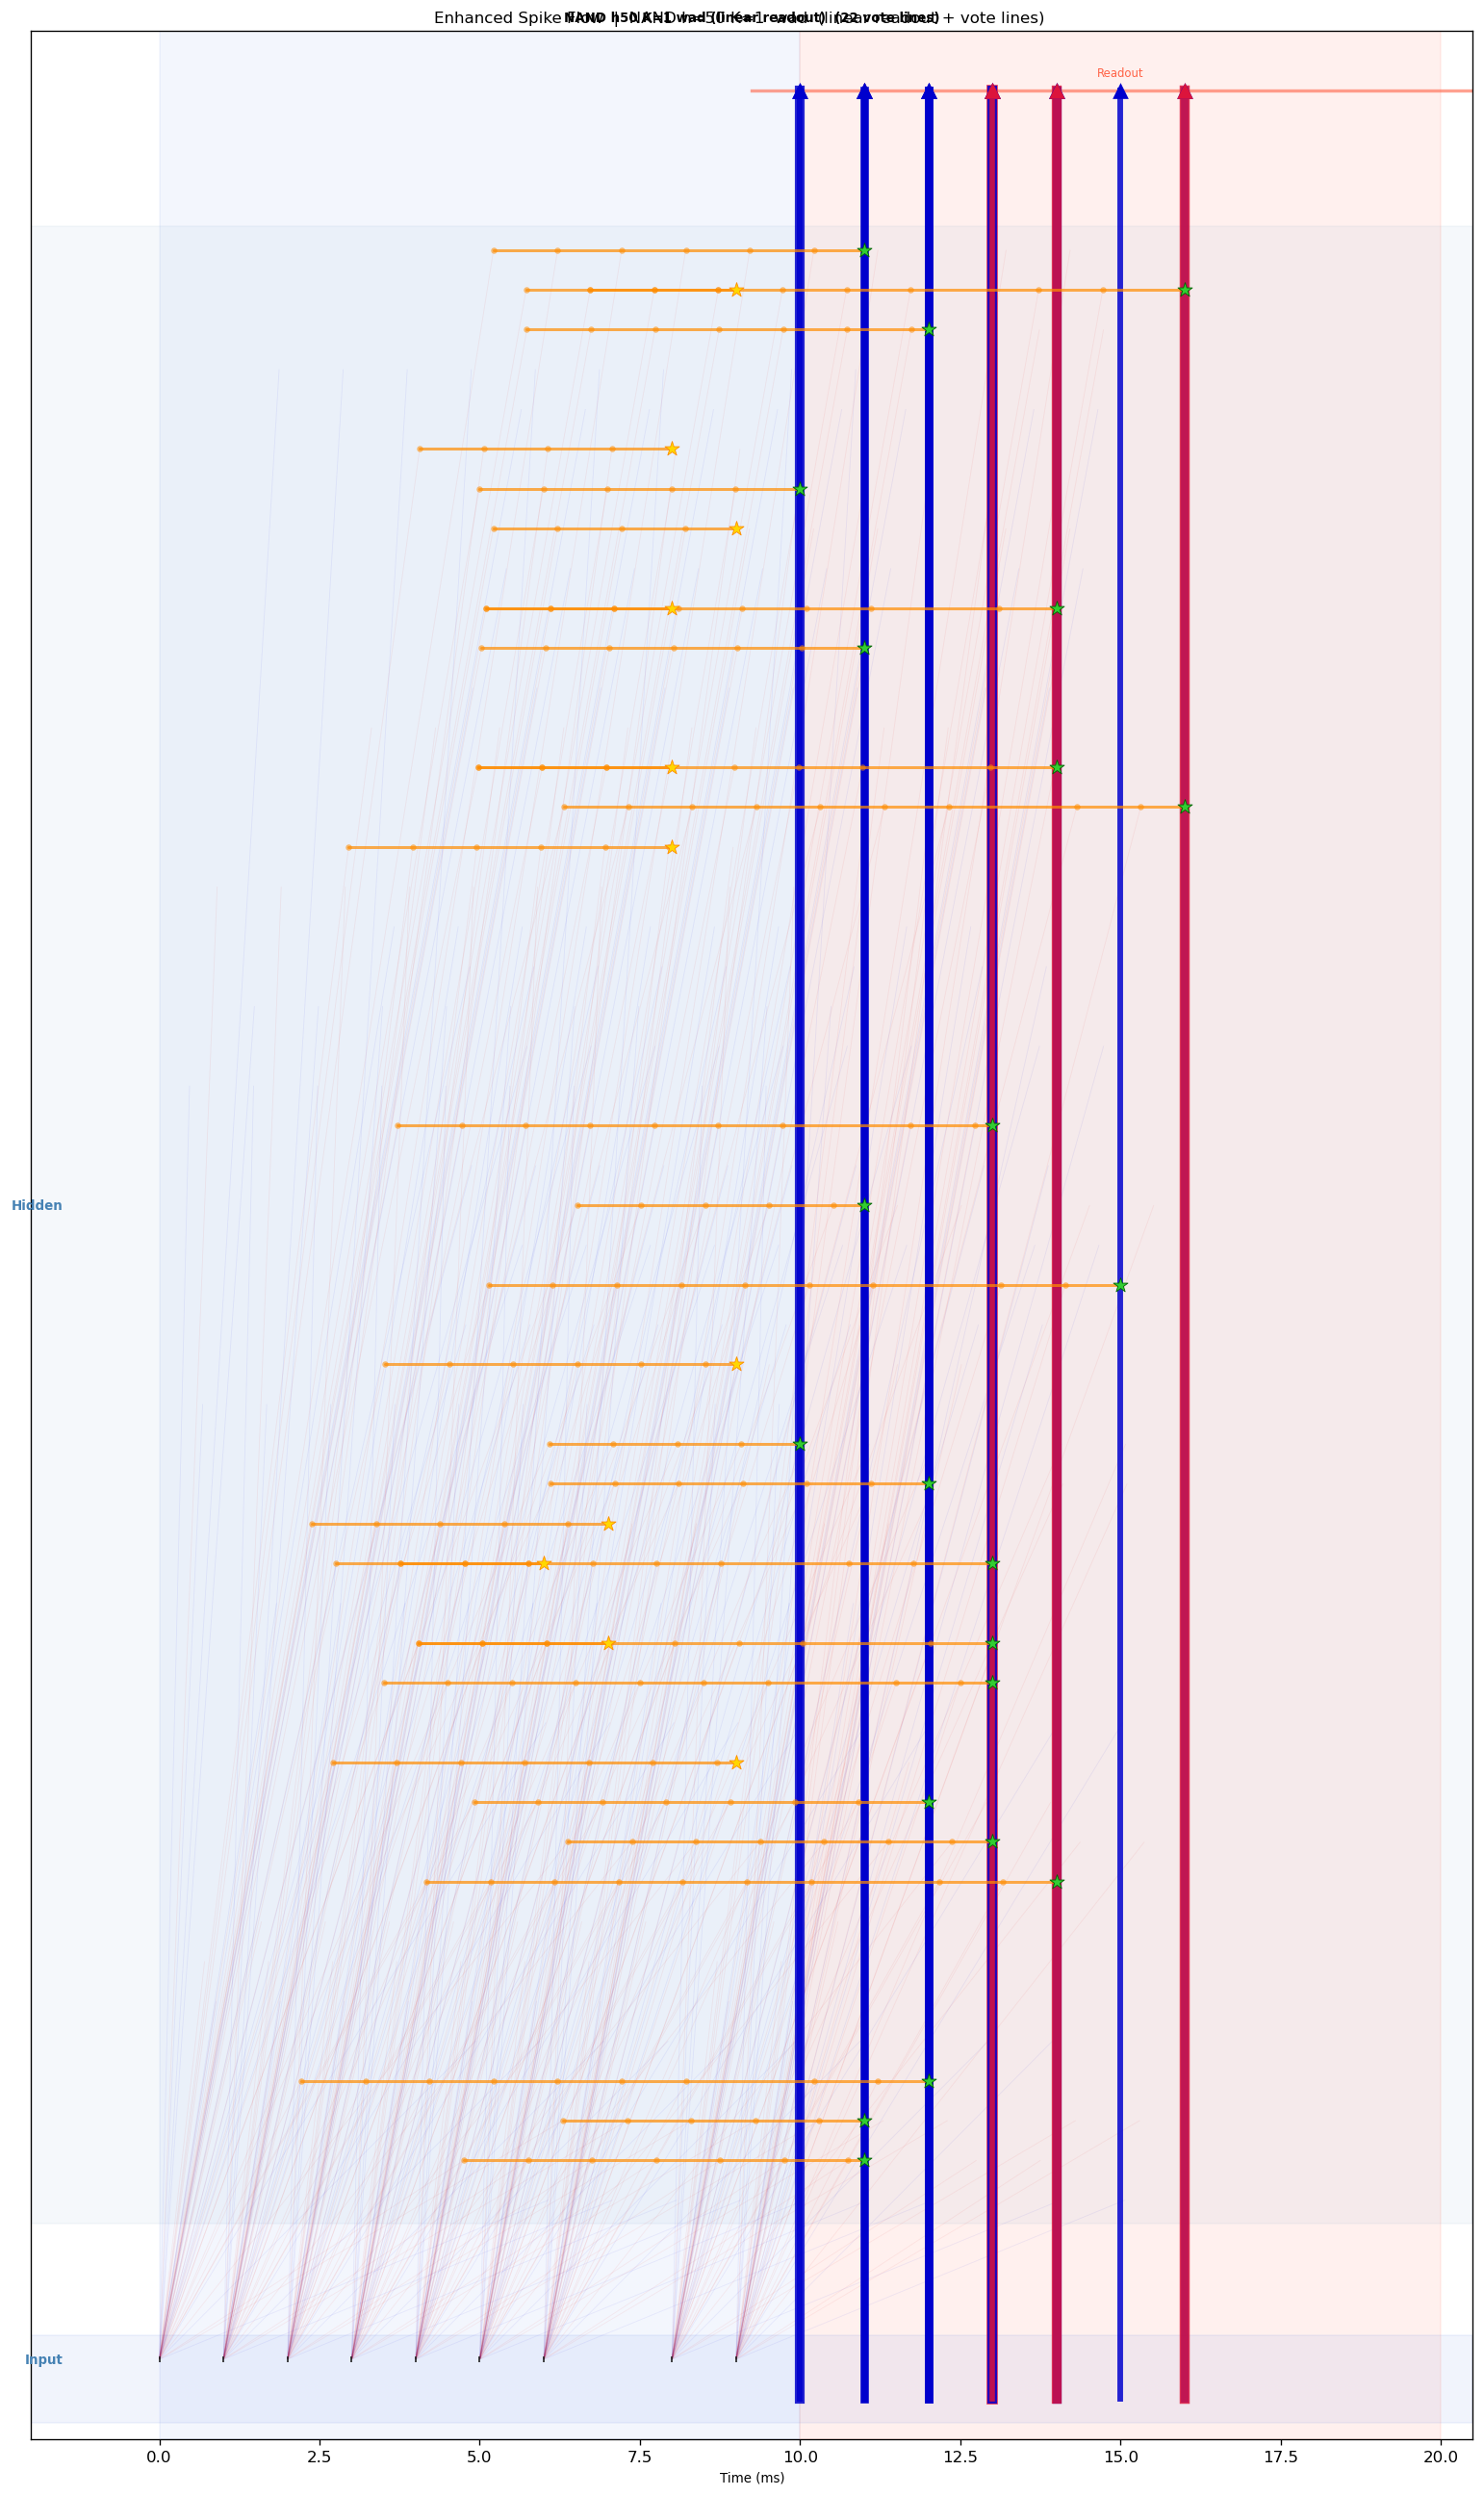
\includegraphics[width=\columnwidth]{fig_method_planD_flow.png}
\caption{SC-design mechanism (NAND, $h{=}50$, $K{=}1$, \texttt{weights\_and\_delays},
linear readout). Three connection types are drawn explicitly: (A) red/blue fan lines
trace every input spike to its delayed arrival at each hidden neuron; (B) orange spans
mark the most recent arrivals that drove a hidden neuron to fire, with the fire itself
shown as a gold star (inside the input window, not yet counted) or a green star (inside
the shared readout window, counted); (C) crimson/blue vertical bars connect
readout-window fires to the linear readout, coloured by the sign of the learned readout
weight. This is the structural mechanism the rest of Section \ref{sec:step2} analyses
quantitatively.}
\label{fig:method}
\end{figure}

\section{Single-Operation Baseline}
\label{sec:step1}

Before testing multi-query designs we confirmed that each training mode can reliably
solve a single query, sweeping 8 boolean operations $\times$ 3 modes $\times$
$h\in\{10,20,50\}$ (200 epochs, seed 42).

\begin{table}[t]
\centering
\caption{Single-operation baseline: accuracy by training mode (mean over 8 ops $\times$ 3 $h$ values).}
\label{tab:step1mode}
\begin{tabular}{lcccc}
\toprule
Mode & Mean & Min & Max & Runs $\geq$95\% \\
\midrule
\texttt{weights\_only} & 0.878 & 0.769 & 0.940 & 0/24 \\
\texttt{delays\_only} & 0.737 & 0.517 & 0.892 & 0/24 \\
\texttt{weights\_and\_delays} & \textbf{0.954} & 0.846 & 0.989 & \textbf{15/24} \\
\bottomrule
\end{tabular}
\end{table}

\begin{table}[t]
\centering
\caption{Single-operation baseline: accuracy by mode $\times$ hidden size.}
\label{tab:step1h}
\begin{tabular}{lccc}
\toprule
$h$ & \texttt{w\_only} & \texttt{d\_only} & \texttt{w\_and\_d} \\
\midrule
10 & 0.853 & 0.706 & \textbf{0.924} \\
20 & 0.888 & 0.753 & \textbf{0.962} \\
50 & 0.893 & 0.753 & \textbf{0.974} \\
\bottomrule
\end{tabular}
\end{table}

\texttt{weights\_and\_delays} dominates at every $h$, with a 7--8 percentage-point gap
over \texttt{weights\_only} that holds across hidden sizes; \texttt{delays\_only}
collapses on XOR/XNOR (mean 0.584 vs.\ 0.800 on the simpler operations), confirming that
delays alone cannot implement the nonlinear decision boundary XOR requires. At $h{=}50$,
NAND reaches 0.989 and was selected as the operation used for all multi-query experiments
below, for its stability; XOR is the
hardest operation at 0.932 (just below the 95\% threshold), setting a difficulty floor.
As a side effect, \texttt{weights\_and\_delays} uses 19\% fewer spikes per trial than
\texttt{weights\_only} at $h{=}50$ (27.7 vs.\ 34.1) while achieving higher accuracy.
Fig.~\ref{fig:step1delay} shows the delay matrix learned for NAND at $h{=}50$: delays
spread over a wide range (2--24 steps) rather than collapsing to a single value,
consistent with different hidden neurons specialising to different latencies.

\begin{figure}[t]
\centering
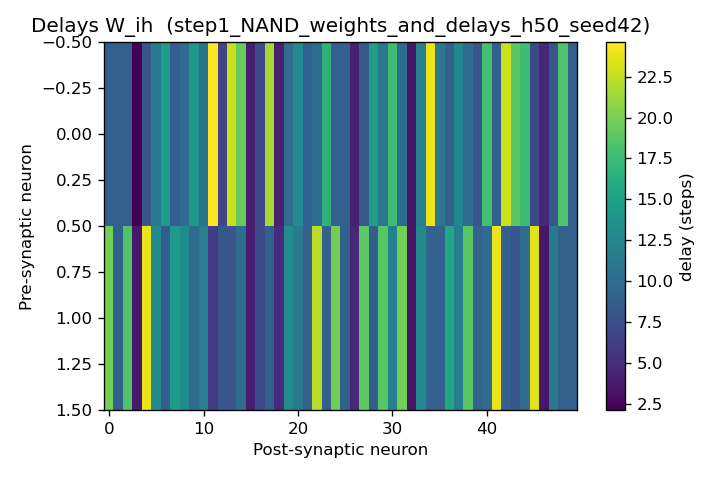
\includegraphics[width=\columnwidth]{fig_step1_delay_heatmap.png}
\caption{Learned input$\to$hidden delay matrix, NAND, $h{=}50$,
\texttt{weights\_and\_delays}.}
\label{fig:step1delay}
\end{figure}

\section{Multi-Query Design Comparison}
\label{sec:step2}

\subsection{Sequential-Readout (SR) design -- serial time slots}

Each of $K$ queries is given its own $35\,\mathrm{ms}$ slot (20 ms input, 10 ms readout, 5
ms gap); trial length grows as $K\times35\,\mathrm{ms}$. \texttt{weights\_and\_delays}
sustains $\geq$95\% accuracy from $K{=}1$ to at least $K{=}20$ with no visible ceiling,
while the $d{=}0$ control cannot even solve $K{=}1$ reliably (79.7\%).

This result is striking but, on inspection, \emph{not} evidence of multiplexing. The
$d{=}0$ failure at $K{=}1$ occurs because the input window ends at 20 ms while the
readout window opens at 20 ms: by then the membrane potential of a delay-free network has
decayed to $e^{-20/10}\approx13\%$ of its peak. Trained delays fix this by shifting input
spikes into the readout window (median learned delay $\tilde d\approx9$ steps) -- this is
\emph{temporal alignment}, not multiplexing. The fact that $K$ scales to 20 without
degradation follows because LIF decay ($\tau_m{=}10\,\mathrm{ms} \ll$ slot length
$35\,\mathrm{ms}$, residual $e^{-3.5}\approx3\%$) provides natural slot isolation --
serial processing of $K$ independent single-query problems, not a shared
representation. \textbf{Lesson:} the SR design cannot test true temporal multiplexing because
each query has its own independent readout.

\subsection{Dedicated-Channel (DC) design -- synchronous channels}

To quantify alignment vs.\ capacity directly, the DC design injects all $K$ queries
simultaneously, each on its own dedicated channel pair ($2K$ input channels total), with
trial length fixed at 30 ms regardless of $K$. Three conditions are compared: (A)
\texttt{weights\_and\_delays}; (B) \texttt{weights\_only} with delays fixed at 20 ms
(alignment without adaptivity); (C) \texttt{weights\_only} with $d{=}0$ (no alignment, no
adaptivity).

\begin{table}[t]
\centering
\caption{DC design: three-condition decomposition (NAND, $h{=}20$).}
\label{tab:planc}
\begin{tabular}{lccccc}
\toprule
$K$ & A (w\&d) & B ($d{=}20$) & C ($d{=}0$) & B$-$C & A$-$B \\
\midrule
1 & 0.973 & 0.957 & 0.801 & 0.156 & 0.016 \\
2 & 0.952 & 0.929 & 0.774 & 0.155 & 0.023 \\
4 & 0.932 & 0.894 & 0.770 & 0.125 & 0.037 \\
6 & 0.899 & 0.866 & 0.769 & 0.097 & 0.033 \\
8 & 0.886 & 0.865 & 0.760 & 0.105 & 0.022 \\
12 & 0.866 & 0.855 & 0.759 & 0.096 & 0.011 \\
\bottomrule
\end{tabular}
\end{table}

The B$-$C column (\emph{alignment effect}) averages $+11.8\%$; the A$-$B column
(\emph{capacity effect}, what adaptive delay adds on top of fixed alignment) averages only
$+2.7\%$ -- a $4.3\times$ ratio. In Max K@90\% terms: fully trainable reaches $K{=}5$,
fixed-alignment reaches $K{=}3$, zero-delay reaches $K{=}0$. The capacity effect is small
here because each query already has a dedicated channel pair: weights alone can route
the right channel to the right output, so delay's marginal contribution is small. This
motivates the SC design: remove the dedicated channels entirely and force the network to rely on
timing alone.

\subsection{Shared-Channel (SC) design -- single shared readout}
\label{sec:pland}

The SC design is the central experiment. Only two input channels (A, B) are shared across all
$K$ queries; query $k$ is injected in sub-window $[k\!\cdot\!\text{sw}, (k\!+\!1)\!\cdot\!\text{sw})$
(sw $=10\,\mathrm{ms}$), and a single shared readout window follows all $K$ sub-windows,
outputting $K$ logits via \texttt{Linear($h$,$K$)}. Because the input weight
$w_{A,j}$ is a single scalar, it responds identically to an $A{=}1$ spike regardless of
\emph{which} sub-window it arrived in -- weights cannot, in principle, distinguish
queries. Only a delay $d_{A,j}\approx\text{win\_len}-k\cdot\text{sw}$ can route query
$k$'s signal to arrive inside the readout window. \textbf{This makes $d{=}0$ a
structural, not merely empirical, failure mode.}

\begin{table}[t]
\centering
\caption{SC design, linear readout: accuracy vs.\ $K$, $h{=}20$ vs.\ $h{=}50$.}
\label{tab:pland}
\begin{tabular}{lccc}
\toprule
$K$ & $h{=}20$ & $h{=}50$ & gap vs.\ $d{=}0$ ($h{=}50$) \\
\midrule
1 & 0.949 & 0.956 & +16.4\% \\
2 & 0.912 & 0.927 & +16.3\% \\
\textbf{3} & 0.835 & \textbf{0.860} & +9.2\% \\
4 & 0.829 & 0.861 & +9.6\% \\
6 & 0.808 & 0.816 & +5.1\% \\
12 & 0.786 & 0.800 & +4.5\% \\
\bottomrule
\end{tabular}
\end{table}

Max K@90\% is \textbf{2} at both $h{=}20$ and $h{=}50$ -- a 150\% increase in neurons
only moves $K{=}3$ accuracy from 83.5\% to 86.0\%, ruling out raw neuron count as the
bottleneck. A 4-seed replication (seeds 0,1,2,42) confirms this is stable: $h{=}50$,
$K{=}2$: $92.20\pm0.75\%$; $K{=}3$: $87.52\pm1.04\%$ (std $<2\%$ throughout).

Figures~\ref{fig:k1} and \ref{fig:k2} show the mechanism directly, via enhanced rasters
(hidden neurons sorted by first-spike time; a dark-red sidebar marks how many of each
neuron's spikes land inside the shared readout window). At $K{=}1$ (Fig.~\ref{fig:k1}),
\texttt{weights\_and\_delays} produces 14 hidden spikes, 9 of which land inside the
readout window (active $12/20$ neurons); $d{=}0$ produces only 2 hidden spikes total
(active $2/20$) -- an order of magnitude less activity, with the network falling back
almost entirely on the readout bias. At $K{=}2$ (Fig.~\ref{fig:k2}),
\texttt{weights\_and\_delays} routes both queries into the readout window (18 hidden
spikes, 8 inside the readout window) via a \emph{query-position delay gradient}: Q0
(earlier) and Q1 (later) use different learned delays so that both signals converge on
overlapping hidden neurons at similar arrival times -- a genuine routing solution. The
$d{=}0$ control is, if anything, \emph{more} active overall (26 hidden spikes, active
$15/20$) but routes \emph{zero} of them into the readout window: every spike is confined
to the two input sub-windows, so the readout decoder receives no signal regardless of
which query is being asked -- a temporal \emph{collision} between Q0 and Q1's
representations, not a lack of computation (accuracy 76.4\% vs.\ 91.2\%). The
input-to-hidden delay matrix for this $K{=}2$ run (Fig.~\ref{fig:k2delay}) confirms this
is not a single global shift: delays cluster into several distinct bands across the 20
hidden neurons rather than one value, consistent with different neurons specialising to
different query-position latencies.

\begin{figure*}[t]
\centering
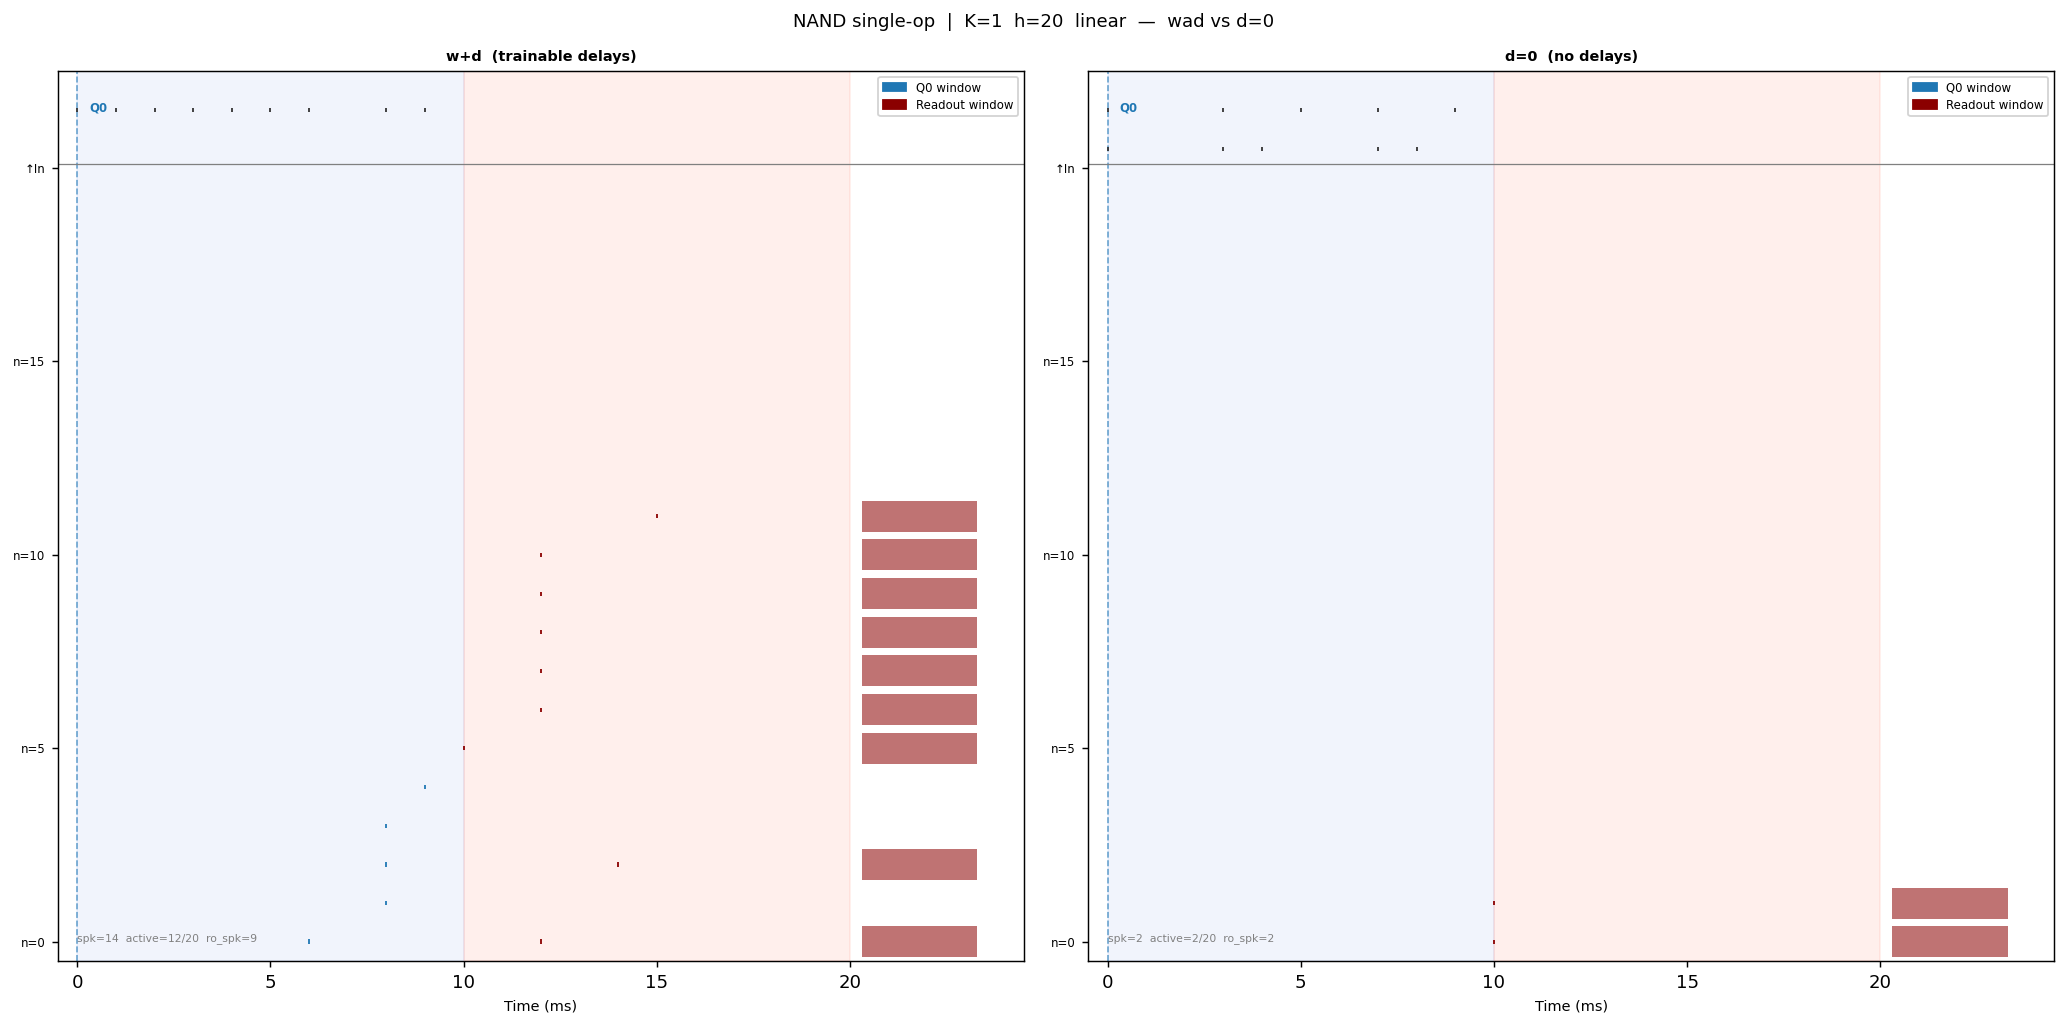
\includegraphics[width=0.85\textwidth]{fig_planD_k1_enhanced.png}
\caption{SC design, $K{=}1$, $h{=}20$: enhanced raster (hidden neurons sorted by
first-spike time, spikes coloured by sub-window), \texttt{weights\_and\_delays} (left,
acc.\ 94.9\%) vs.\ $d{=}0$ (right, acc.\ 76.4\%). With trainable delays a clear band of
neurons fires inside the readout window (dark-red sidebar); with $d{=}0$ the network
falls back on the readout bias.}
\label{fig:k1}
\end{figure*}

\begin{figure}[t]
\centering
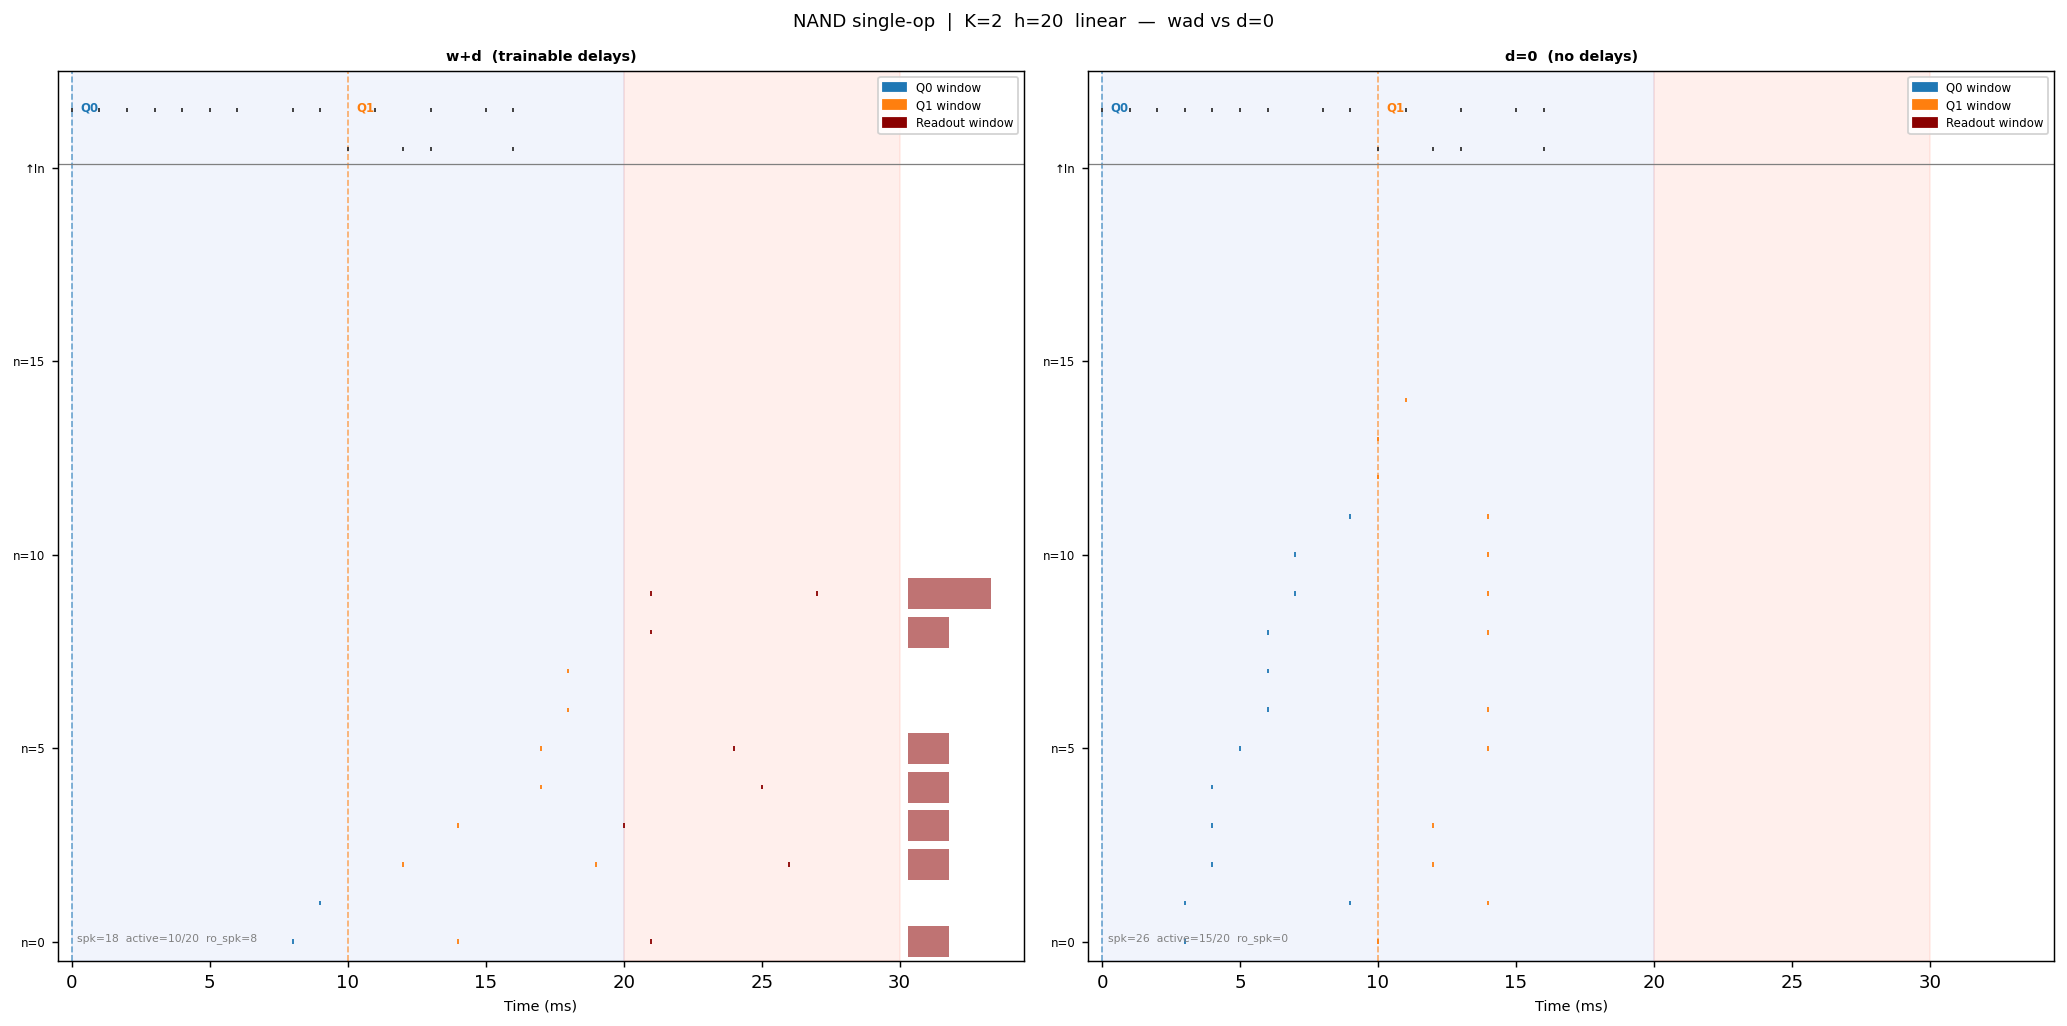
\includegraphics[width=\columnwidth]{fig_planD_k2_enhanced.png}
\caption{SC design, $K{=}2$, $h{=}20$: enhanced raster, \texttt{weights\_and\_delays}
(left, 91.2\%) vs.\ $d{=}0$ (right, 76.4\%). With delays, Q0 (long delay) and Q1 (short
delay) converge on overlapping hidden neurons inside the readout window; with $d{=}0$,
both queries arrive at the same neurons at the same time -- a temporal collision rather
than a routing failure.}
\label{fig:k2}
\end{figure}

\begin{figure}[t]
\centering
\begin{subfigure}{0.48\columnwidth}
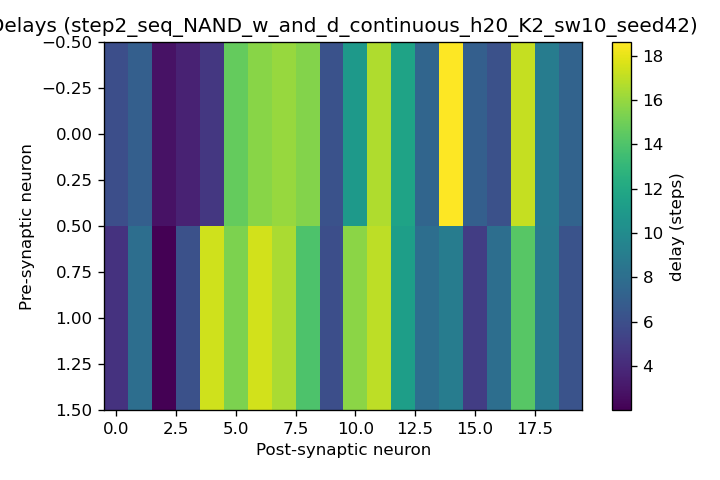
\includegraphics[width=\linewidth]{fig_planD_k2_delayheatmap.png}
\caption{Delay matrix}
\end{subfigure}
\hfill
\begin{subfigure}{0.48\columnwidth}
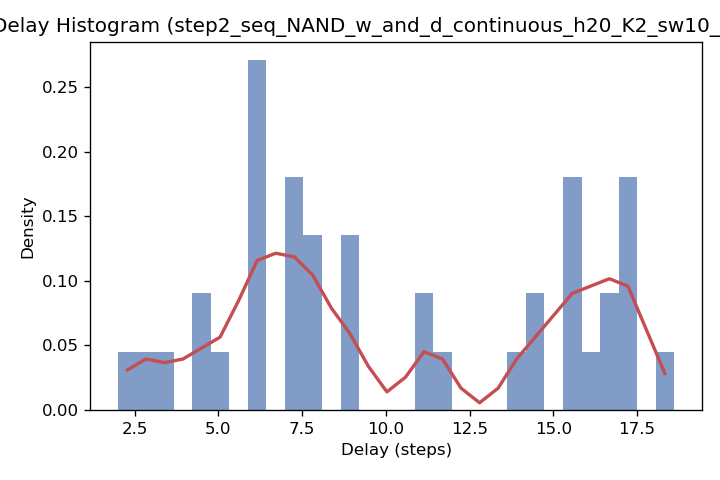
\includegraphics[width=\linewidth]{fig_planD_k2_delayhist.png}
\caption{Delay distribution}
\end{subfigure}
\caption{Learned input$\to$hidden delays for the $K{=}2$, $h{=}20$,
\texttt{weights\_and\_delays} run of Fig.~\ref{fig:k2}. Rather than collapsing to a
single value, delays cluster into several distinct bands across the 20 hidden neurons,
consistent with different neurons specialising to different query-position latencies
rather than learning one global alignment offset.}
\label{fig:k2delay}
\end{figure}

\section{Ablations and Causal Isolation}
\label{sec:ablation}

\subsection{MLP readout breaks the $K{=}2$ ceiling}
Replacing the linear readout with a one-hidden-layer MLP
(\texttt{Linear($h,h$)$\to$ReLU$\to$Linear($h,K$)}) lifts $K{=}3$ accuracy from 87.52\%
(linear) to 92.68\% (MLP, mean of 2 seeds, both $>$92\%), crossing the 90\% threshold and
advancing \textbf{Max K@90\% from 2 to 3}. Fig.~\ref{fig:k3} shows the underlying enhanced
spike-flow diagrams (fan lines = input$\to$hidden arrivals, orange spans = integration
windows that drove a fire, stars = fire time). The linear panel (left) carries its
decision through a small number of explicit crimson/blue \emph{vote lines} -- thick
vertical bars where a readout-window fire is weighted and summed. The MLP panel (right)
has no such single weighted channel: it instead recruits visibly \emph{more} hidden
neurons whose fires land inside the readout window (green stars), with the
linear-vs-nonlinear transform distributing the decision across all of them rather than
any one weighted vote -- consistent with the network exploiting overlapping,
non-linearly-separable temporal codes that a linear decoder cannot extract.

These two readouts, plus a third we tried, trade off accuracy against
interpretability and trainability. \textbf{Linear} readout gives each hidden neuron a
single weighted vote (Eq.~\eqref{eq:loss}'s $z$ is one dot product), is cheapest and most
interpretable (Fig.~\ref{fig:k3}'s vote lines are literally the readout weights), but can
only extract linearly-separable structure from the hidden code, capping Max K@90\% at 2.
\textbf{MLP} readout adds one ReLU layer, can extract the non-linearly-separable temporal
codes above, and raises Max K@90\% to 3, at the cost of losing the single-vote-line
interpretation (the decision is distributed across more neurons with no one channel
responsible). We also tried a fully \textbf{spiking output layer} (a third LIF layer
reading the hidden spikes, trained with the same Eq.~\eqref{eq:loss} on its own output
spike count) -- the most hardware-faithful, end-to-end-event-driven option, but the
hardest to train: stacking a second surrogate-gradient nonlinearity on top of the hidden
layer's own surrogate gradient produces a severe dead-neuron problem for the first
$\sim$90 epochs, and even after 1000 epochs it reaches only 71.8\% at $K{=}1$ (vs.\
43.6\% for $d{=}0$, preserving the usual delay gap, but far below the 95\%+ that linear or
MLP readout reach at the same $K$). We therefore use it only for fully-spiking
visualisation (Section~\ref{sec:future}), not as a primary readout.

\begin{figure}[t]
\centering
\begin{subfigure}{0.48\columnwidth}
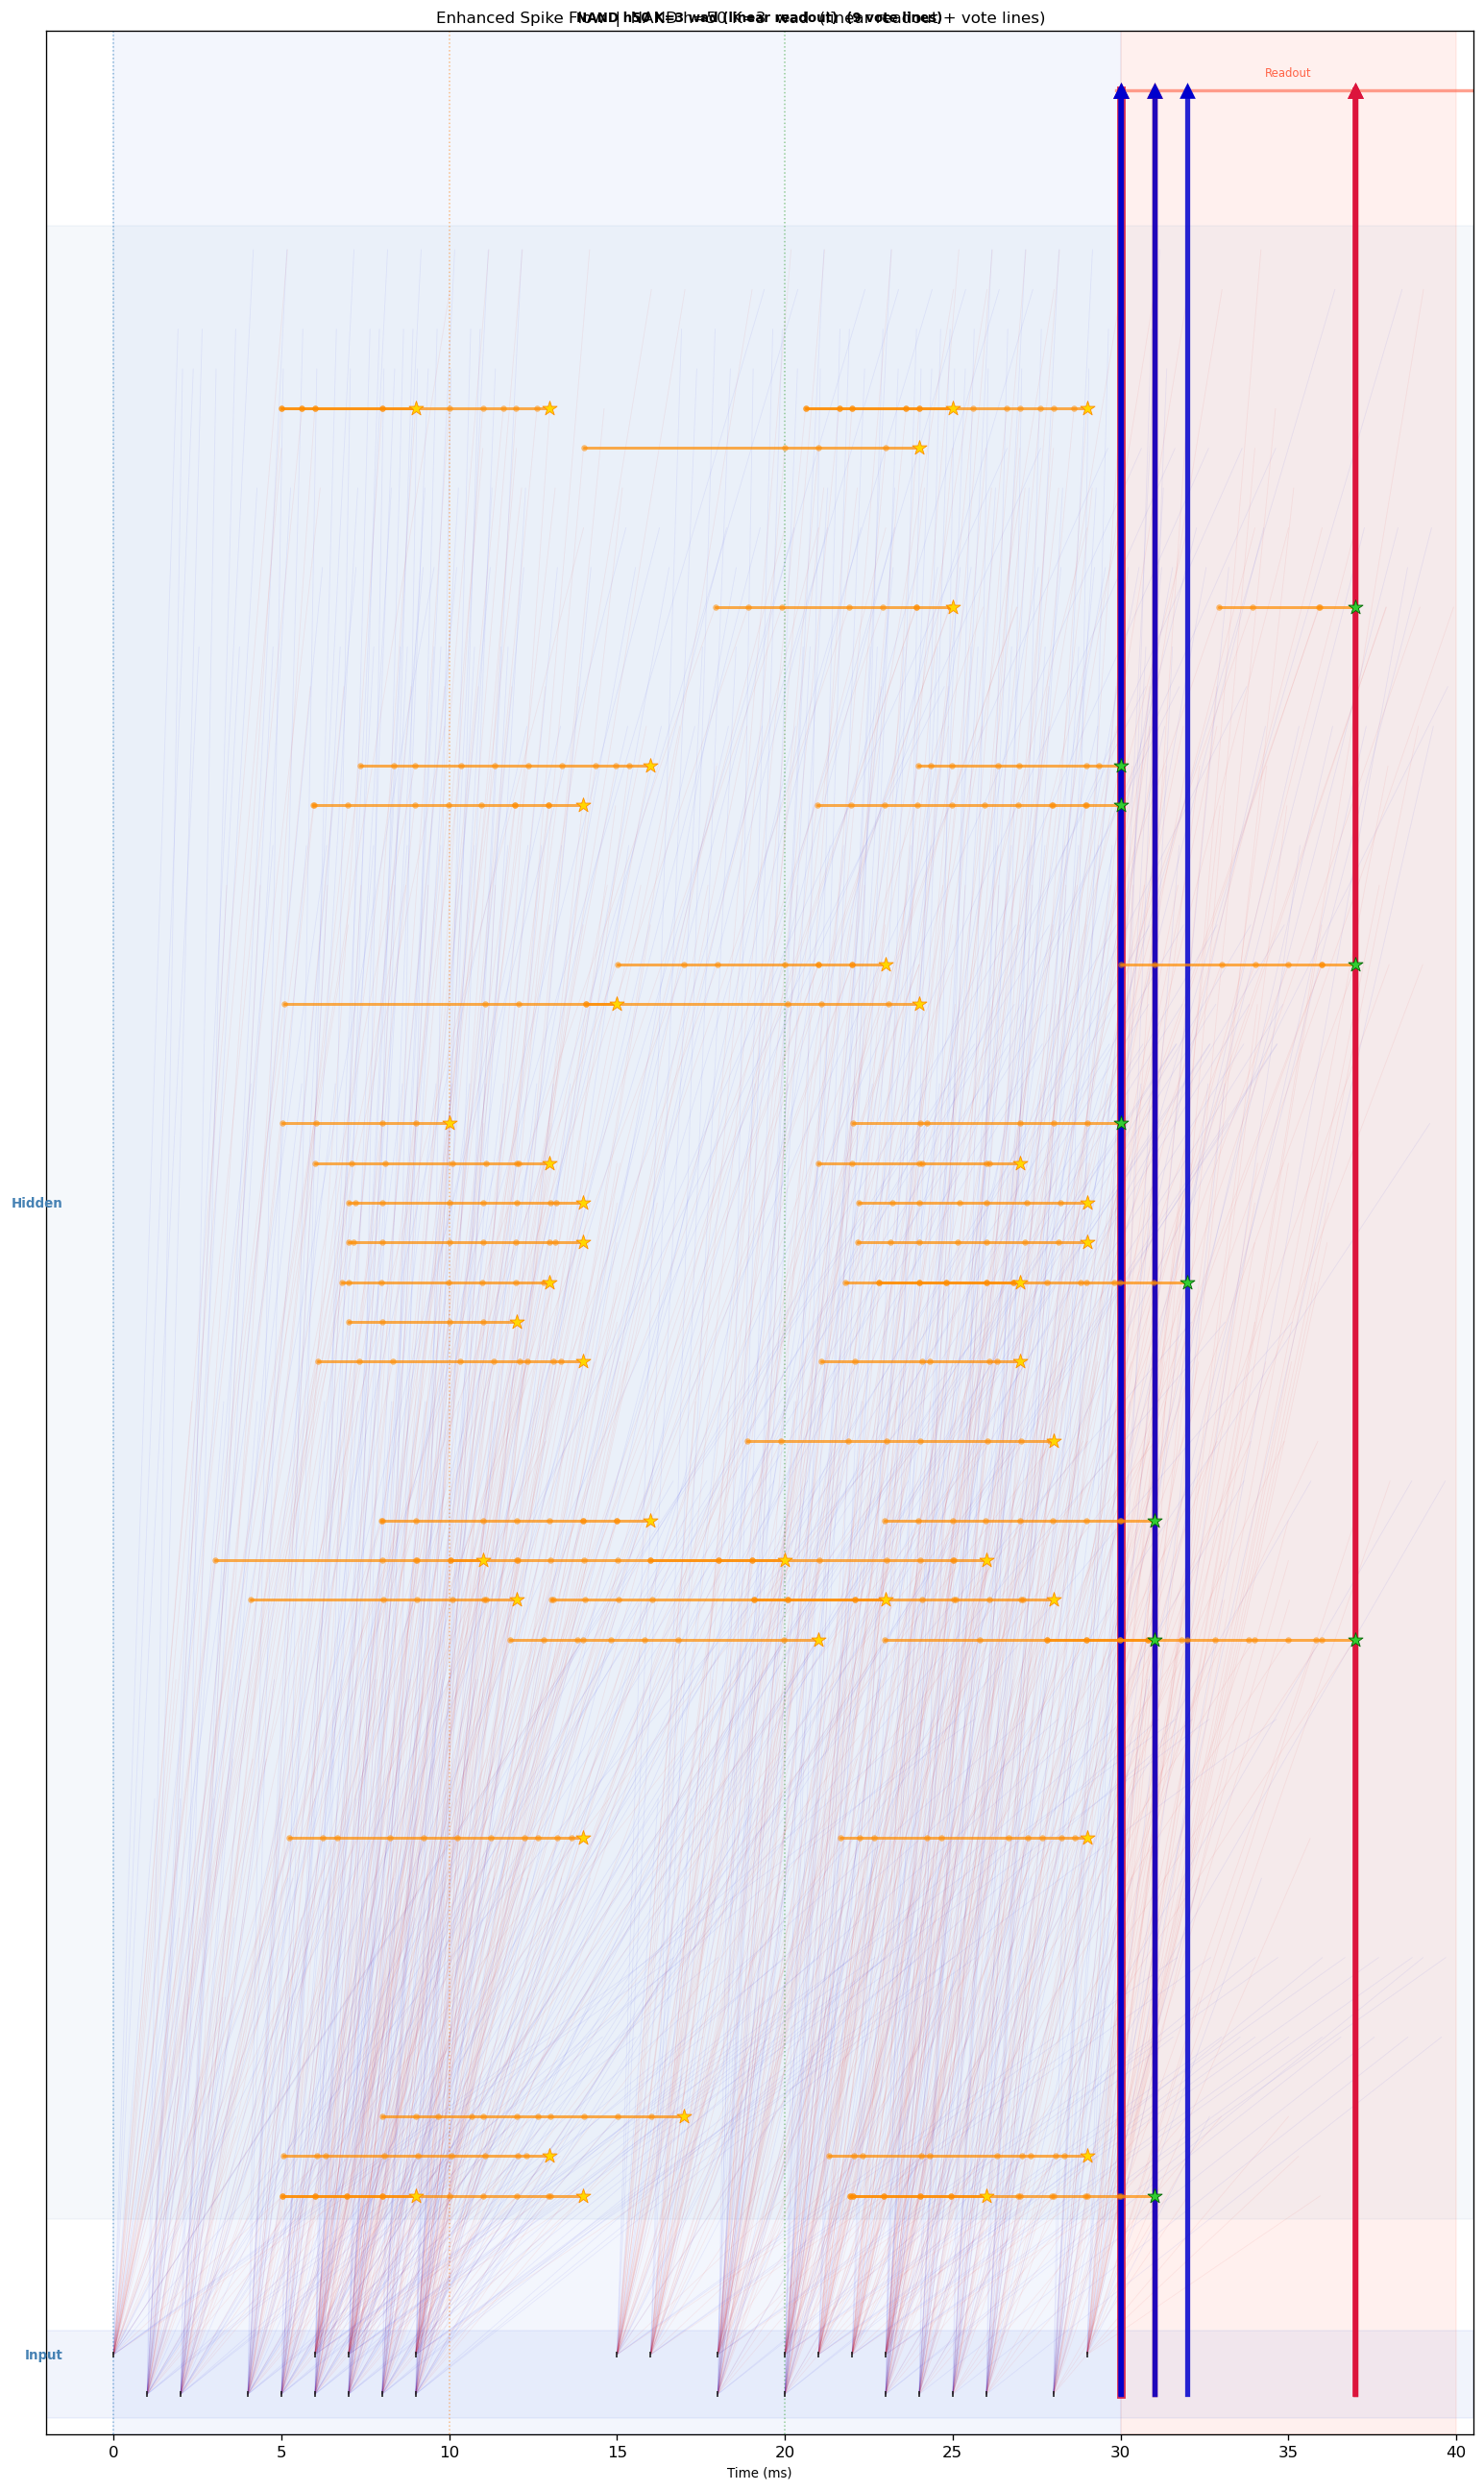
\includegraphics[width=\linewidth]{fig_planD_k3_linear_flow.png}
\caption{Linear (86.0\%)}
\end{subfigure}
\hfill
\begin{subfigure}{0.48\columnwidth}
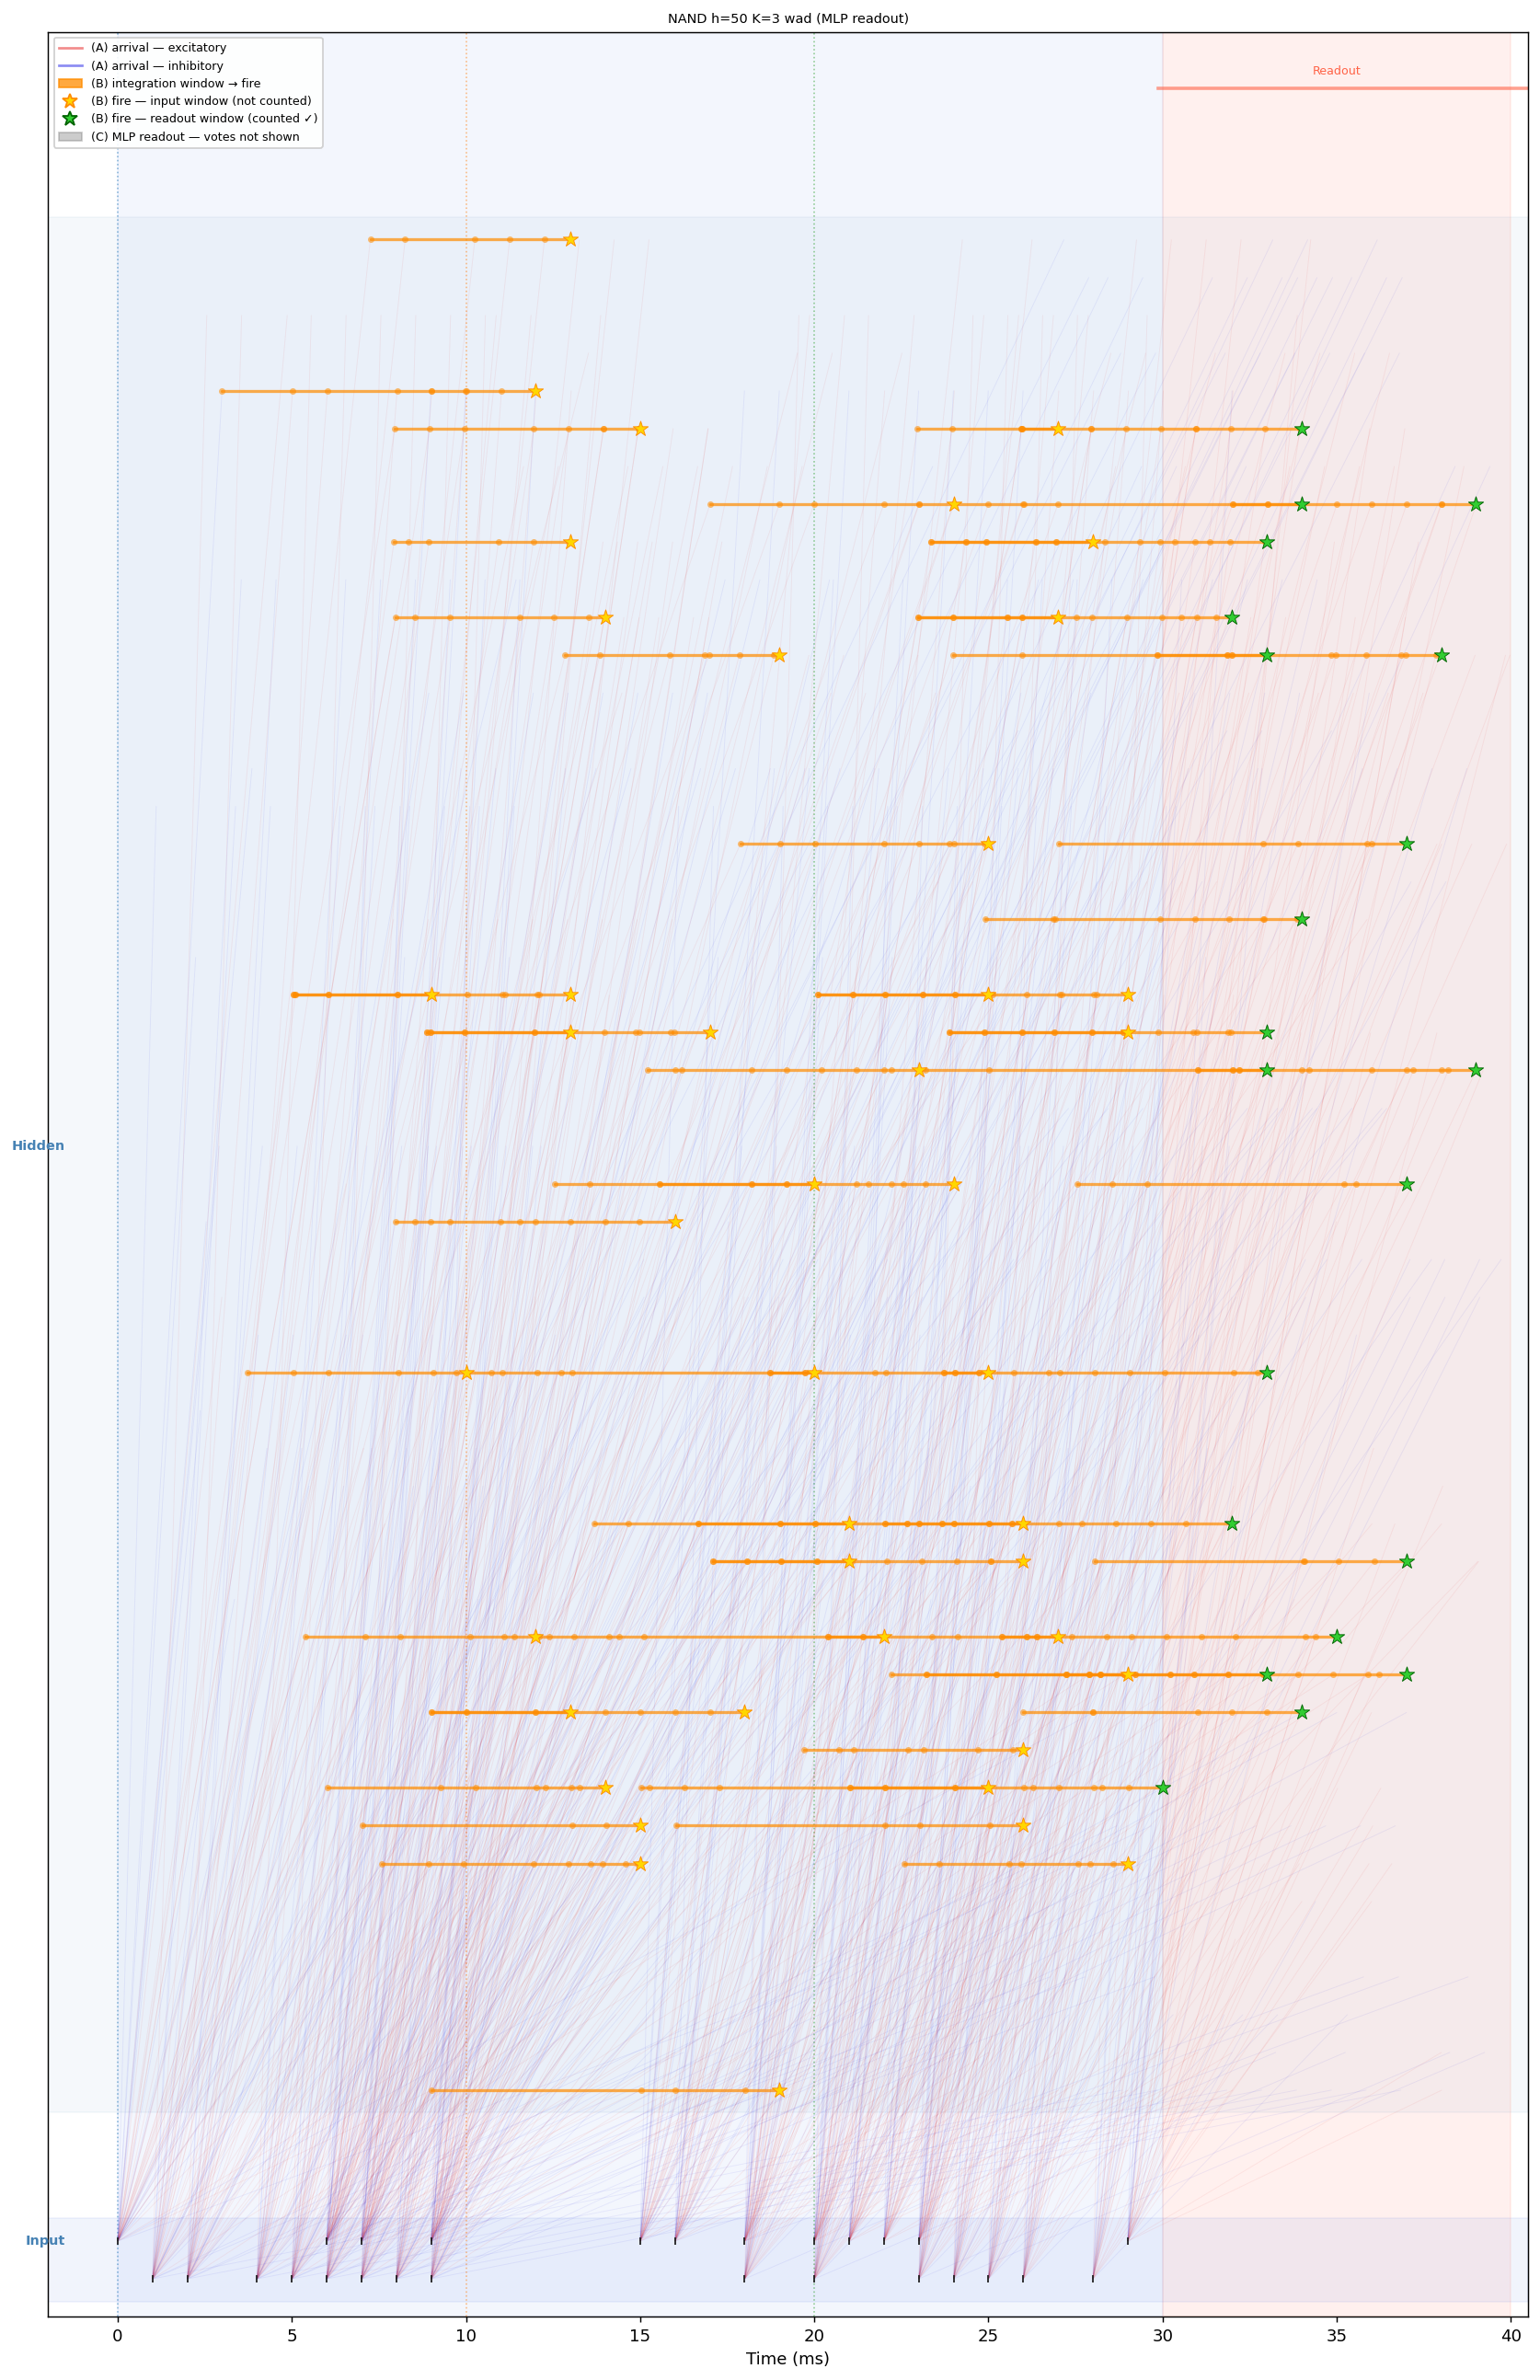
\includegraphics[width=\linewidth]{fig_planD_k3_mlp_flow.png}
\caption{MLP (92.3\%)}
\end{subfigure}
\caption{SC design, $K{=}3$, $h{=}50$, \texttt{weights\_and\_delays}, enhanced spike flow:
linear readout (left, explicit vote lines) vs.\ MLP readout (right, no single weighted
channel -- decision distributed across more readout-window fires, green stars).}
\label{fig:k3}
\end{figure}

\subsection{$2\times2$ causal ablation: is it the delay or the MLP?}
\label{sec:2x2}
The MLP result raises an obvious confound: maybe an MLP alone (without delays) is
powerful enough to solve the task. We rule this out with a full $2\times2$ ablation
(readout $\times$ delay configuration, $h{=}50$):

\begin{table}[t]
\centering
\caption{$2\times2$ ablation: readout type $\times$ delay configuration.}
\label{tab:2x2}
\begin{tabular}{llccc}
\toprule
Readout & Delay & $K{=}2$ & $K{=}3$ & Max K@90\% \\
\midrule
Linear & $d{=}0$ & $\sim$76\% & $\sim$76\% & 0 \\
Linear & trainable & 92.20\% & 87.52\% & 2 \\
MLP & $d{=}0$ & 78.15\% & $\sim$77\% & 0 \\
MLP & trainable & \textbf{93.50\%} & \textbf{92.68\%} & \textbf{3} \\
\bottomrule
\end{tabular}
\end{table}

MLP+$d{=}0$ (77.1\%) is statistically indistinguishable from Linear+$d{=}0$
($\sim$76--77\%): the MLP contributes \emph{nothing} without delays.
Fig.~\ref{fig:abl} confirms this visually, and more precisely than raw spike counts
alone: the MLP+$d{=}0$ flow diagram shows plenty of integration activity (orange spans,
gold stars) \emph{within} each of the three input sub-windows, but across the 20 richest
of 20 sampled trials at most a single hidden fire ever lands inside the shared readout
window -- the same temporal mistiming, not a lack of computation, that Fig.~\ref{fig:k2}
showed for the linear $d{=}0$ control at $K{=}2$. \textbf{Conclusion: the causal driver is
the delay, not the MLP.} The delay effect (trainable vs.\ $d{=}0$) is $\sim$16 percentage
points regardless of readout type; the MLP then adds a further $\sim$5 points \emph{on top
of} delay-created representations, but only once those representations exist.

\begin{figure}[t]
\centering
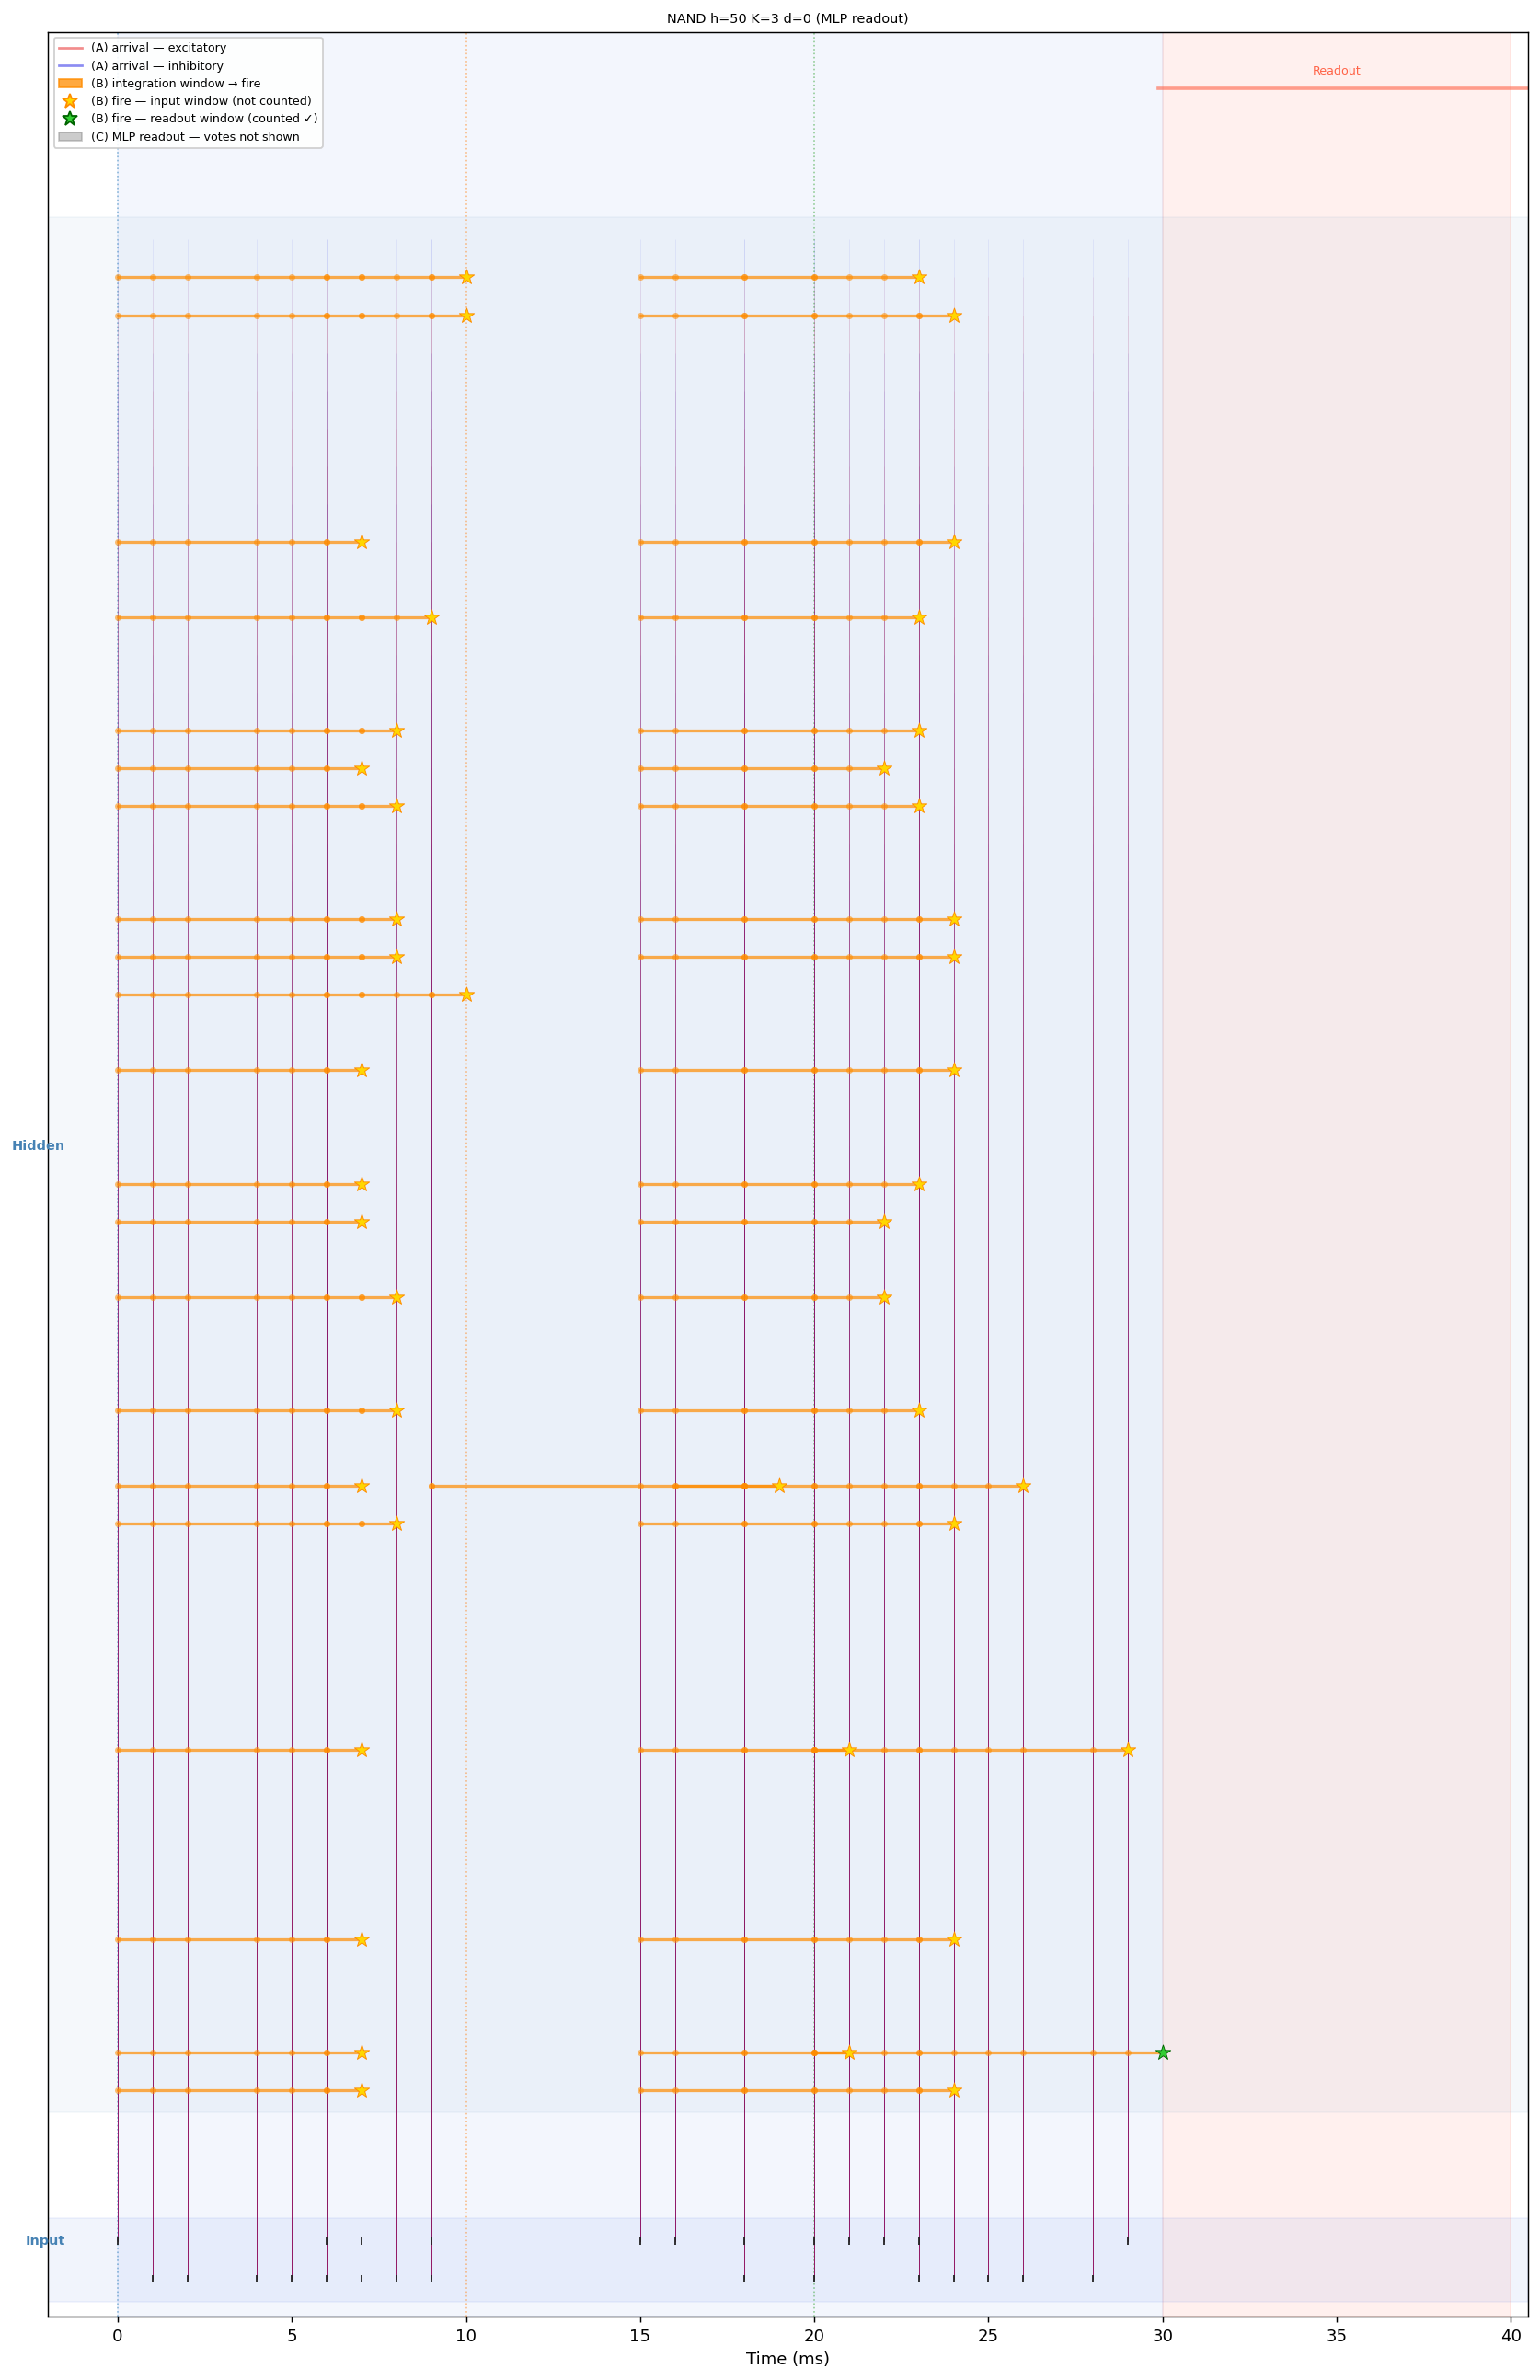
\includegraphics[width=0.8\columnwidth]{fig_ablation_mlp_d0_flow.png}
\caption{MLP readout with $d{=}0$, $K{=}3$, $h{=}50$ (acc.\ 77.1\%), enhanced spike flow:
substantial integration within each input sub-window (orange spans), but at most one
hidden fire reaches the shared readout window across all sampled trials -- the same
alignment failure as the linear $d{=}0$ control, not an absence of activity.}
\label{fig:abl}
\end{figure}

\subsection{Depth ablation: does a second spiking layer help?}
At a fixed 50-neuron total budget, splitting into two spiking layers
($h_1{=}25,h_2{=}25$) does not improve on a single layer ($h{=}50$) for the linear
readout (Max K@90\%$=2$ for both), and for the MLP readout the two-layer variant is
\emph{worse} (Max K@90\%$=2$ vs.\ 3 for one layer) -- depth and MLP gains are not
additive, because the MLP's benefit scales with the dimensionality of the
representation it reads from ($h_2{=}25$ here vs.\ $h{=}50$ for the one-layer case). This
raises an obvious follow-up: is it \emph{depth itself} that is unhelpful, or only depth
\emph{at a fixed budget} that halves the readout's input dimension? We re-ran the
two-layer architecture without the budget constraint -- $h_1{=}50,h_2{=}50$ (100 neurons
total, double the single-layer budget, but $\text{readout\_in}{=}50$ matches the
single-layer case exactly) -- with both readouts, $K\in\{2,3,4\}$, 2 seeds.

\begin{table}[t]
\centering
\caption{Depth ablation, NAND (mean of 2 seeds). Top: fixed 50-neuron budget. Bottom:
unconstrained depth (100 neurons, $\text{readout\_in}{=}50$).}
\label{tab:depth}
\begin{tabular}{lcccc}
\toprule
Model & $K{=}2$ & $K{=}3$ & $K{=}4$ & Max K@90\% \\
\midrule
L1-h50-linear & 92.4\% & 87.3\% & 84.9\% & 2 \\
L1-h50-MLP & 95.9\% & 92.7\% & 89.9\% & 3 \\
L2-h25h25-linear & 91.4\% & 88.6\% & 88.2\% & 2 \\
L2-h25h25-MLP & 91.6\% & 88.3\% & 86.5\% & 2 \\
L2-h25h25-$d{=}0$ & 77.7\% & 77.4\% & 76.9\% & 0 \\
\midrule
L2-h50h50-linear & 93.6\% & 92.5\% & \textbf{91.1\%} & \textbf{4} \\
L2-h50h50-MLP & \textbf{94.6\%} & \textbf{92.0\%} & 89.7\% & 3 \\
\bottomrule
\end{tabular}
\end{table}

\textbf{Unconstrained depth helps substantially.} L2-h50h50-linear reaches 91.1\% at
$K{=}4$ -- \textbf{Max K@90\% rises to 4}, the best result anywhere in this paper for
single-operation NAND, surpassing even L1-h50-MLP (Max K@90\%$=$3). This confirms that
the earlier ``depth hurts'' finding was an artefact of the \emph{fixed-budget}
constraint specifically: depth that adds capacity (rather than splitting existing
capacity) helps, and helps more than swapping in a nonlinear readout at the original
budget. We do not have a single-layer $h{=}100$ control for single-operation NAND (the
analogous comparison exists only for the mixed-operation task, Section \ref{sec:step3},
where it also reaches Max K@90\%$=$3), so we cannot yet fully attribute this gain to
depth \emph{per se} as opposed to simply having twice the neurons; disentangling the two
is flagged as a remaining experiment in Section~\ref{sec:future}.

A second, unexpected result: at $K{=}4$, \textbf{the linear readout now beats the MLP
readout} (91.1\% vs.\ 89.7\%), reversing the pattern seen everywhere else in this paper.
We interpret this as the two spiking layers' own layer-to-layer nonlinearity (the
LIF spike function in $h_1\to h_2$) already supplying much of the non-linear separability
that the MLP readout was previously needed to extract from a single spiking layer; adding
a further non-spiking nonlinearity on top of two spiking layers does not help further,
and its extra parameters ($\mathrm{Linear}(50,50)\to\mathrm{ReLU}\to\mathrm{Linear}(50,4)$
vs.\ $\mathrm{Linear}(50,4)$) may mildly overfit the fixed 4000-trial training set.

Fig.~\ref{fig:depthraster} additionally shows the raw raster for the linear-readout
single-vs-two-layer comparison at $K{=}3$ (fixed-budget case): the two architectures
produce qualitatively similar (sparse, query-staggered) hidden activity, consistent with
the fixed-budget conclusion that depth alone does not change the qualitative mechanism --
delays still do the routing, as in Section \ref{sec:2x2}. The $d{=}0$ control collapses to
$\sim$77\% regardless of depth, confirming delays remain the necessary mechanism
independent of architecture. Fig.~\ref{fig:depthcurve} shows the corresponding
accuracy/throughput-vs-$K$ curves for the two-layer MLP variant (fixed-budget case):
accuracy degrades gracefully but stays below the 90\% threshold from $K{=}3$ onward,
while energy-normalised throughput is non-monotonic (0.072 $\to$ 0.084 $\to$ 0.082),
reflecting the same capacity-boundary effects discussed in Section \ref{sec:pland}.

\begin{figure*}[t]
\centering
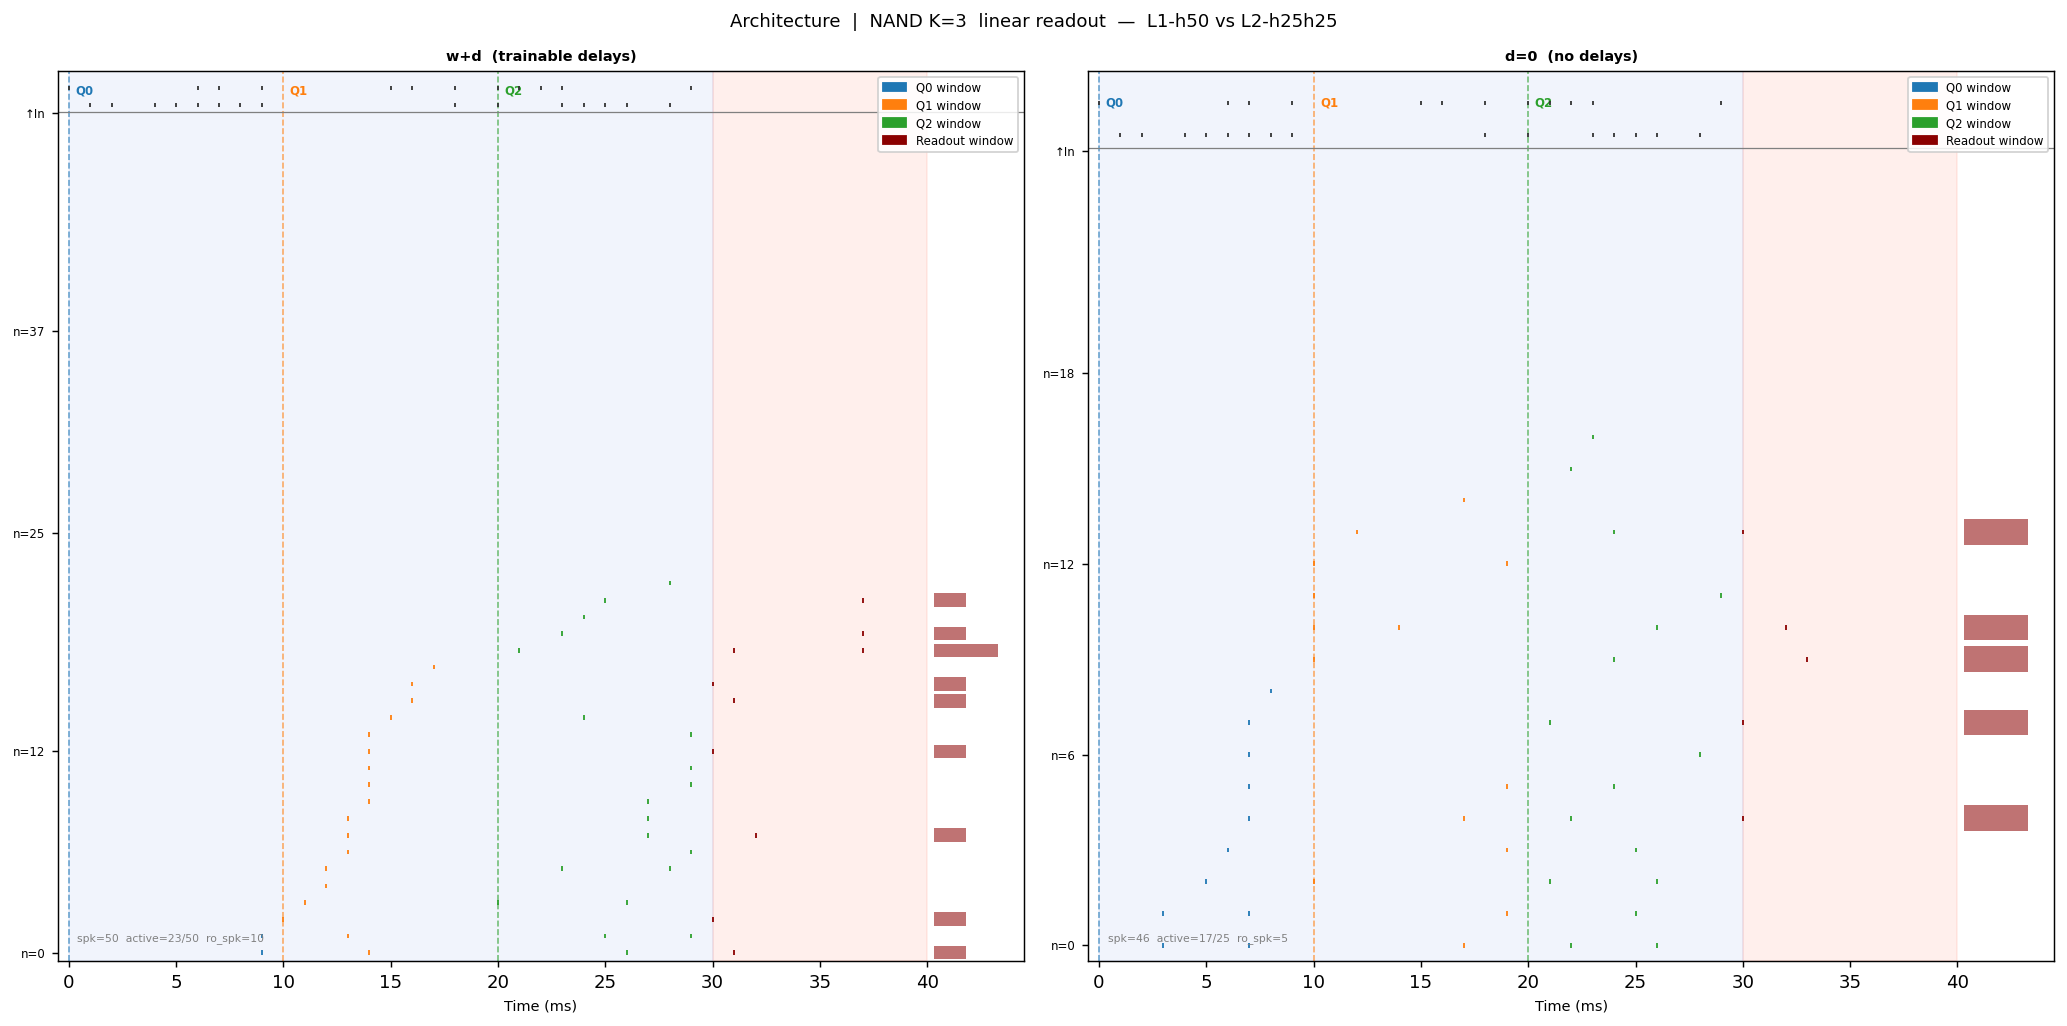
\includegraphics[width=0.85\textwidth]{fig_step3_depth.png}
\caption{Depth ablation raster, NAND, $K{=}3$, linear readout: $h{=}50$ single layer
(left) vs.\ $h_1{=}25,h_2{=}25$ two layers (right), trainable delays.}
\label{fig:depthraster}
\end{figure*}

\begin{figure*}[t]
\centering
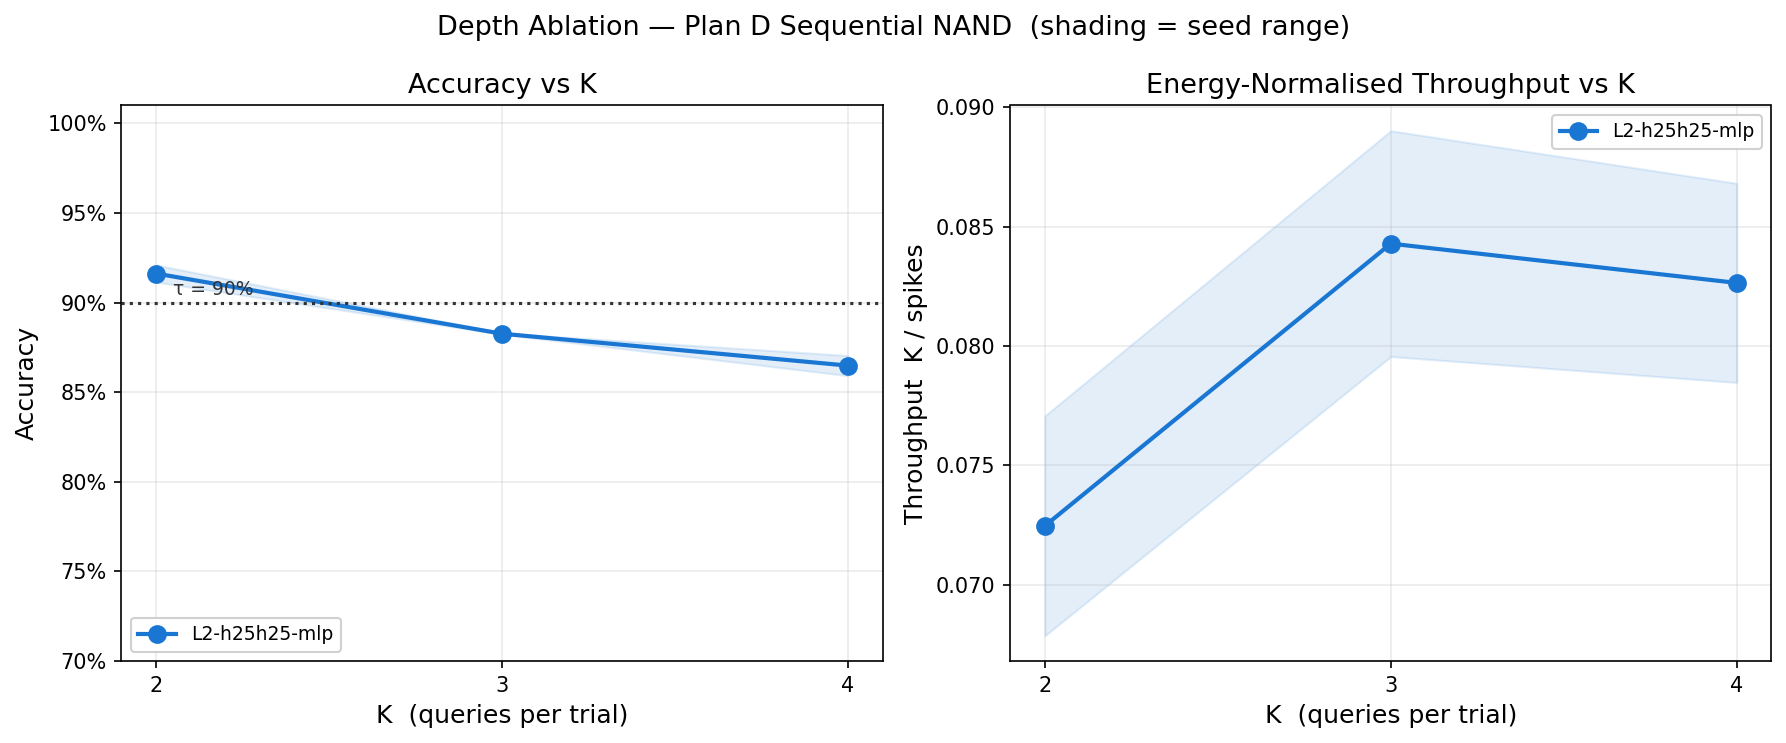
\includegraphics[width=0.7\textwidth]{fig_depth_ablation.png}
\caption{Two-layer MLP variant (L2-h25h25-MLP): accuracy and energy-normalised throughput
vs.\ $K$, shading shows seed range.}
\label{fig:depthcurve}
\end{figure*}

\subsection{Timing-parameter ablation}
We tested whether the $K{=}3$ ceiling is a fixable timing artefact -- specifically,
whether $\text{sub\_win}=\tau_m=10\,\mathrm{ms}$ causes query 0's signal to decay by
$\approx$63\% before the readout window opens. We swept sub-window length, readout-window
length, and $\tau_m$ (one at a time, plus a combined condition), all on the best-known
architecture (L1-h50+MLP+delay).

\begin{table}[t]
\centering
\caption{Timing ablation (L1-h50+MLP+delay, baseline Max K@90\%=3).}
\label{tab:timing}
\begin{tabular}{lcccc}
\toprule
Condition & sw & read\_len & $\tau_m$ & $K{=}3$ / Max K@90\% \\
\midrule
baseline & 10 & 10 & 10.0 & \textbf{92.7\%} / \textbf{3} \\
read\_len20 & 10 & 20 & 10.0 & 91.3\% / 3 \\
subwin5 & 5 & 10 & 10.0 & 85.2\% / 0 \\
tau20 & 10 & 10 & 20.0 & 88.6\% / 0 \\
combined & 5 & 20 & 20.0 & 82.6\% / 0 \\
\bottomrule
\end{tabular}
\end{table}

Every intervention performs at or below baseline; none breaks the ceiling. To see why, we
re-ran a forward pass from the saved \texttt{baseline}, \texttt{tau20}, and
\texttt{combined} checkpoints ($K{=}3$) and compared the richest-of-20 sampled trial for
each (Fig.~\ref{fig:timingflow}). Raising $\tau_m$ does \emph{not} simply make neurons
fire less overall: total hidden spikes barely change (39 baseline vs.\ 35 for both
\texttt{tau20} and \texttt{combined}). What changes is \emph{when} they fire. Counting
spikes by sub-window (Q0/Q1/Q2), baseline concentrates input-phase activity in the
\emph{last} sub-window before the shared readout window opens (0/3/15 spikes); both
\texttt{tau20} and \texttt{combined} shift this activity systematically \emph{earlier}
(0/9/10 and 0/6/10) -- slower membrane decay lets each query's signal persist into the
\emph{next} query's sub-window, exactly the cross-query bleed the natural-slot-isolation
argument warns about. This earlier firing comes directly at the expense of the readout
window: spikes landing inside it drop from 21 (baseline) to 16 (\texttt{tau20}, $-24\%$)
and 19 (\texttt{combined}), with active readout-contributing neurons falling from 20 to
16 and 17 respectively. The mean arrival-to-fire integration span for readout-window
fires is essentially unchanged across conditions (8.0--8.9 simulation steps), confirming
this is a \emph{timing-shift}, not a wholesale collapse of integration dynamics: raising
$\tau_m$ \emph{weakens} the natural slot isolation the SR design relied
on by letting one query's representation leak into the next, increasing cross-query
interference rather than reducing information; shrinking the sub-window (\texttt{subwin5},
\texttt{combined}) compounds this by giving rate-coded inputs less time to generate
spikes in the first place. \textbf{The $K{=}3$ ceiling is not a tunable timing artefact}
-- it survives retuning of every timing constant in the simulation.

\begin{figure*}[t]
\centering
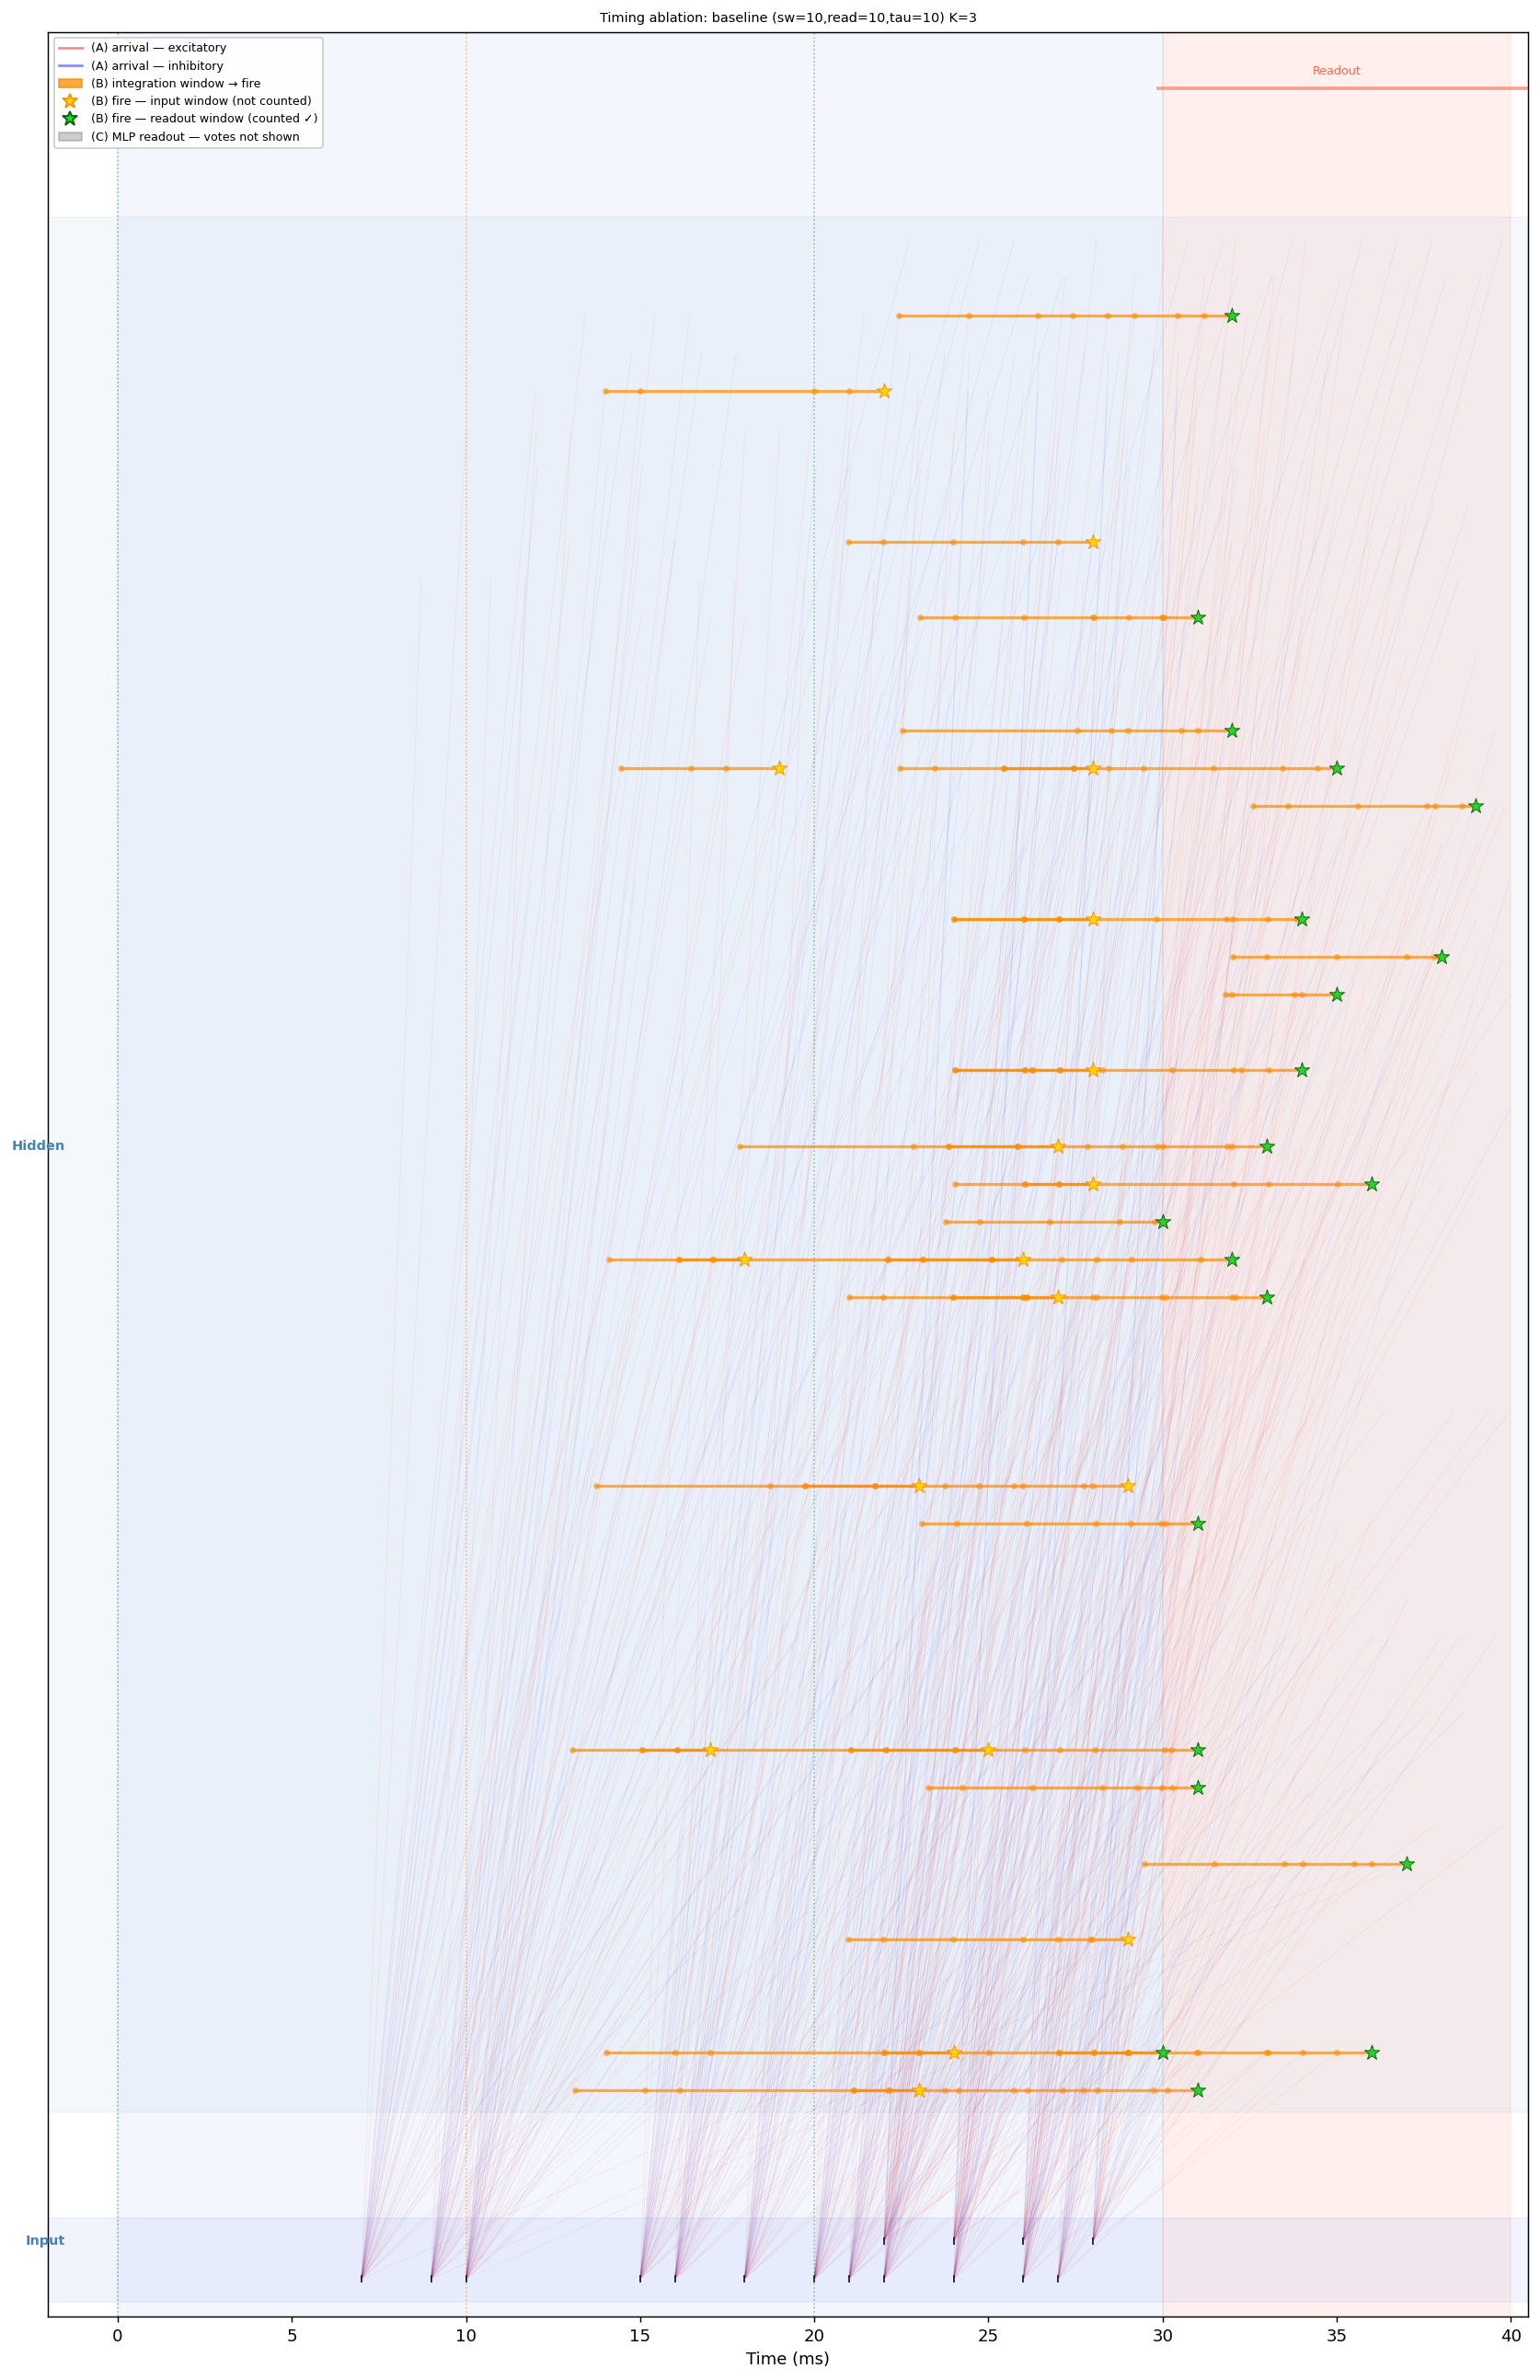
\includegraphics[width=0.31\textwidth]{timing_baseline_K3_flow.png}\hfill
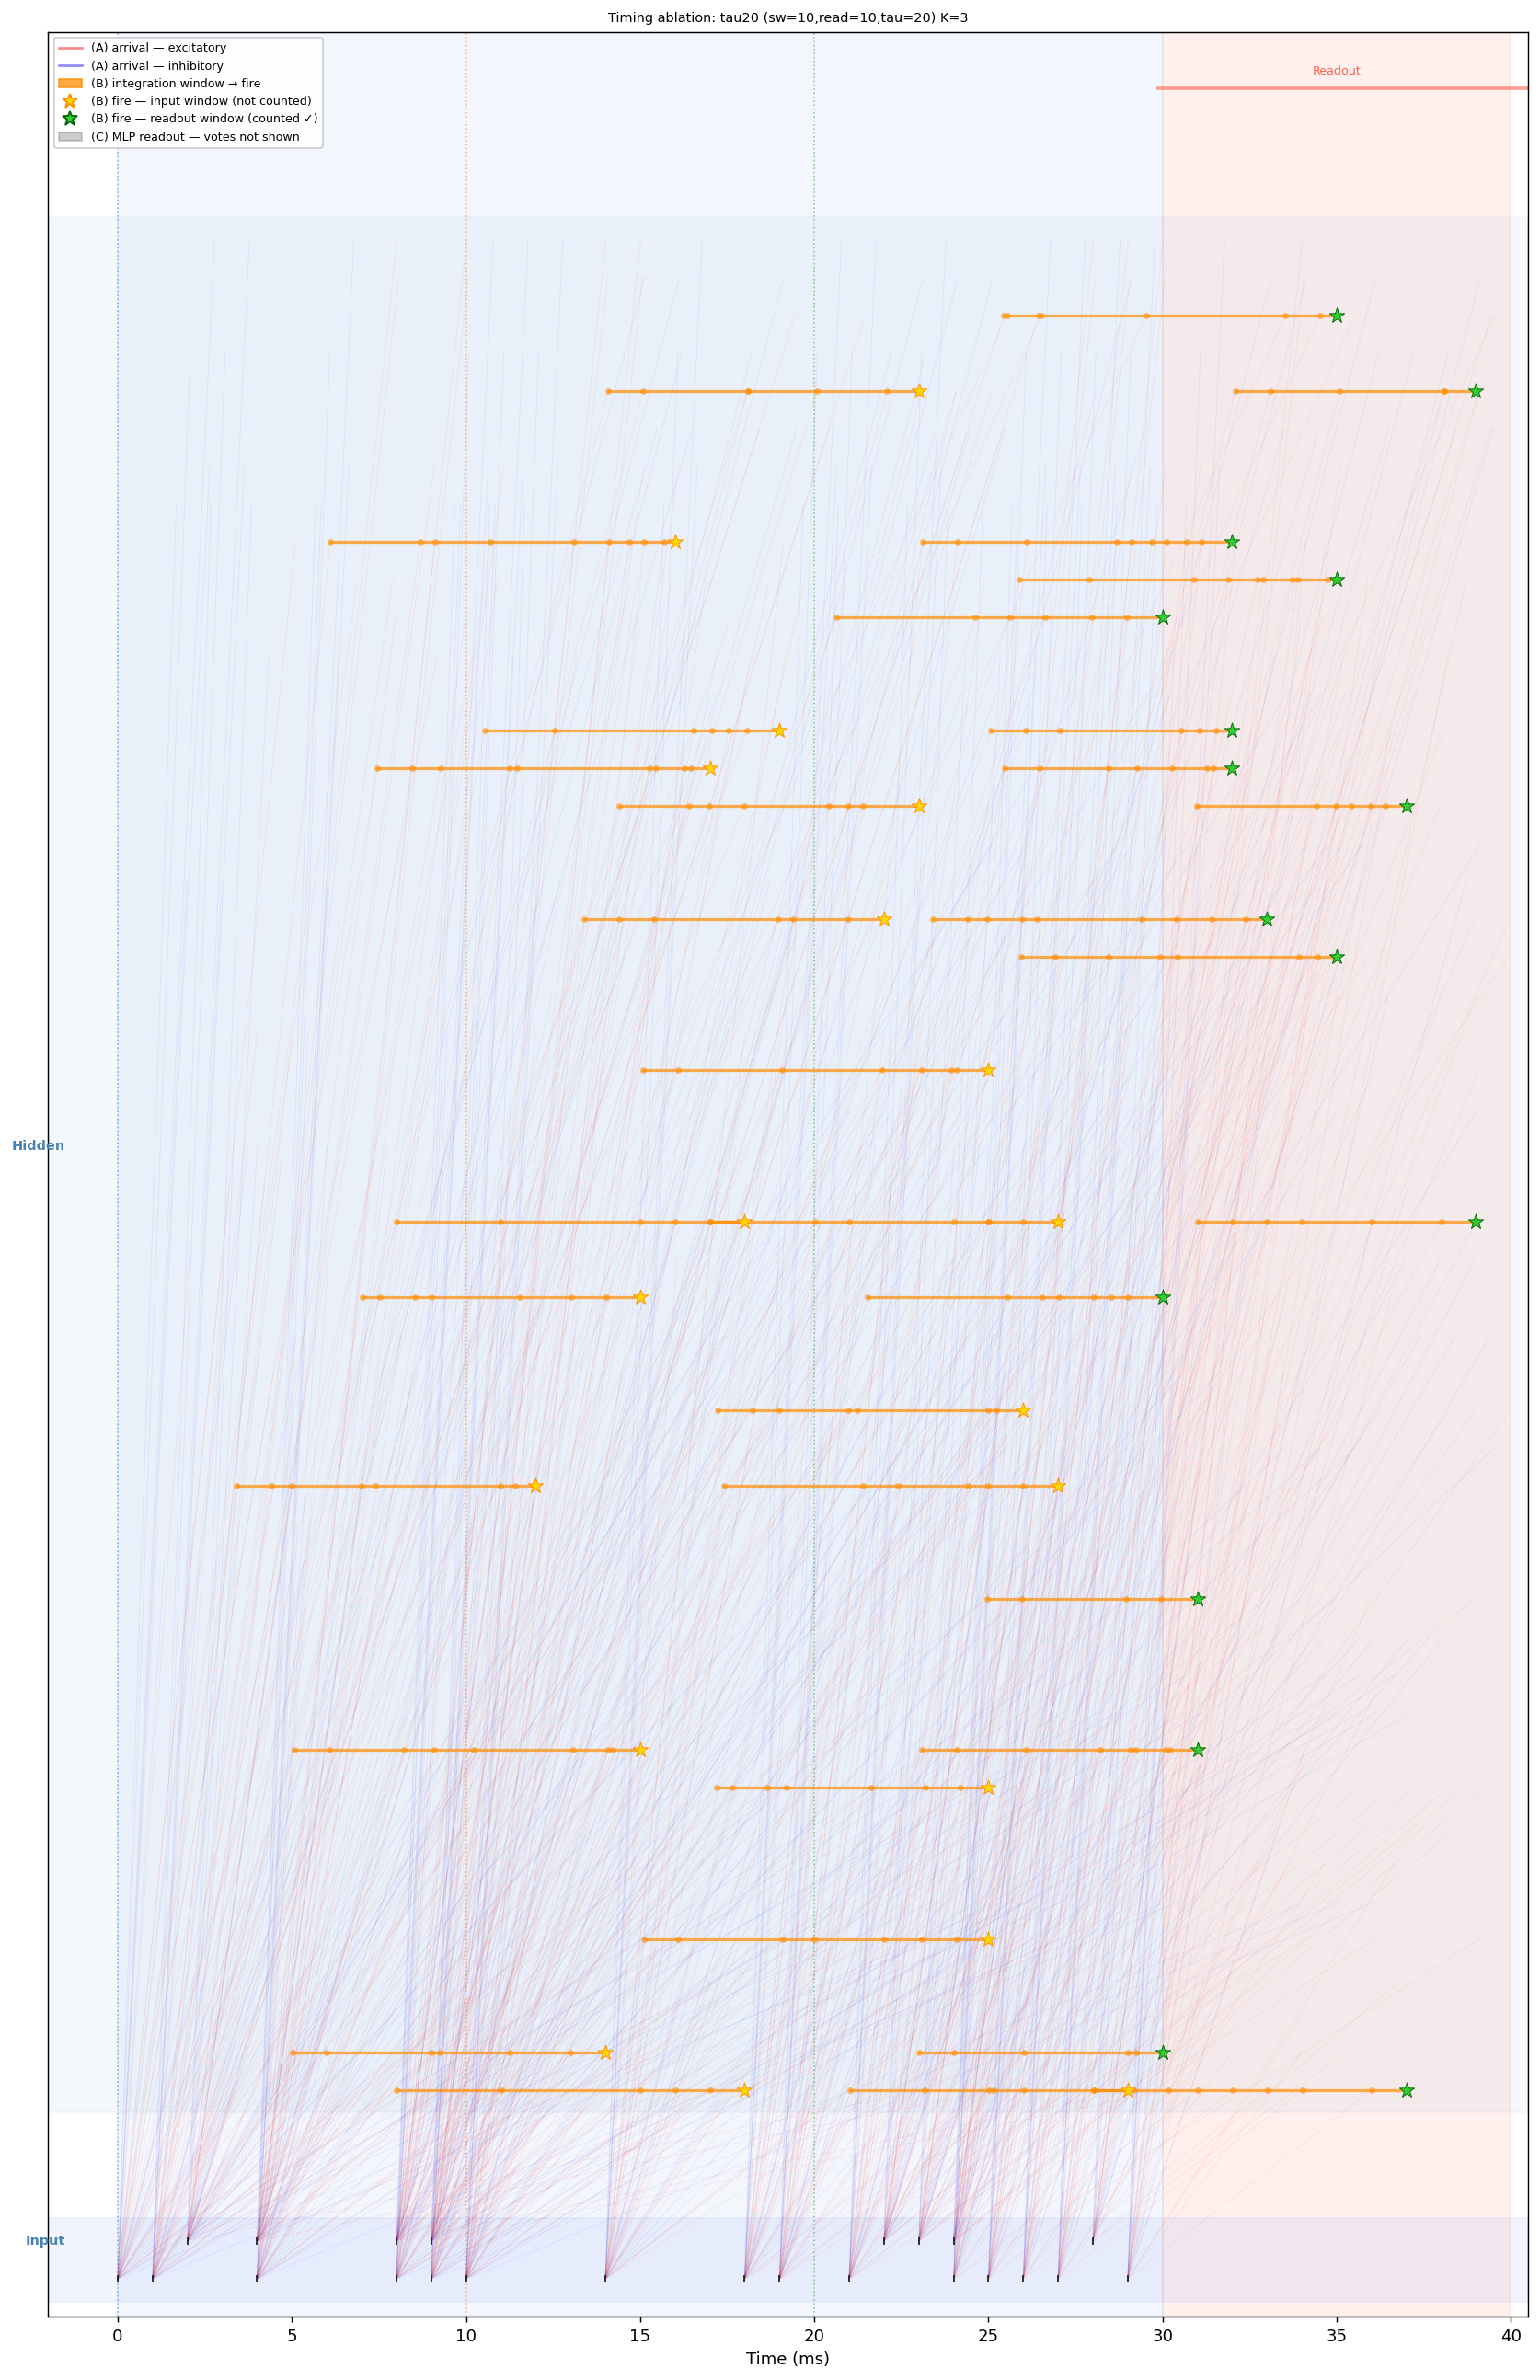
\includegraphics[width=0.31\textwidth]{timing_tau20_K3_flow.png}\hfill
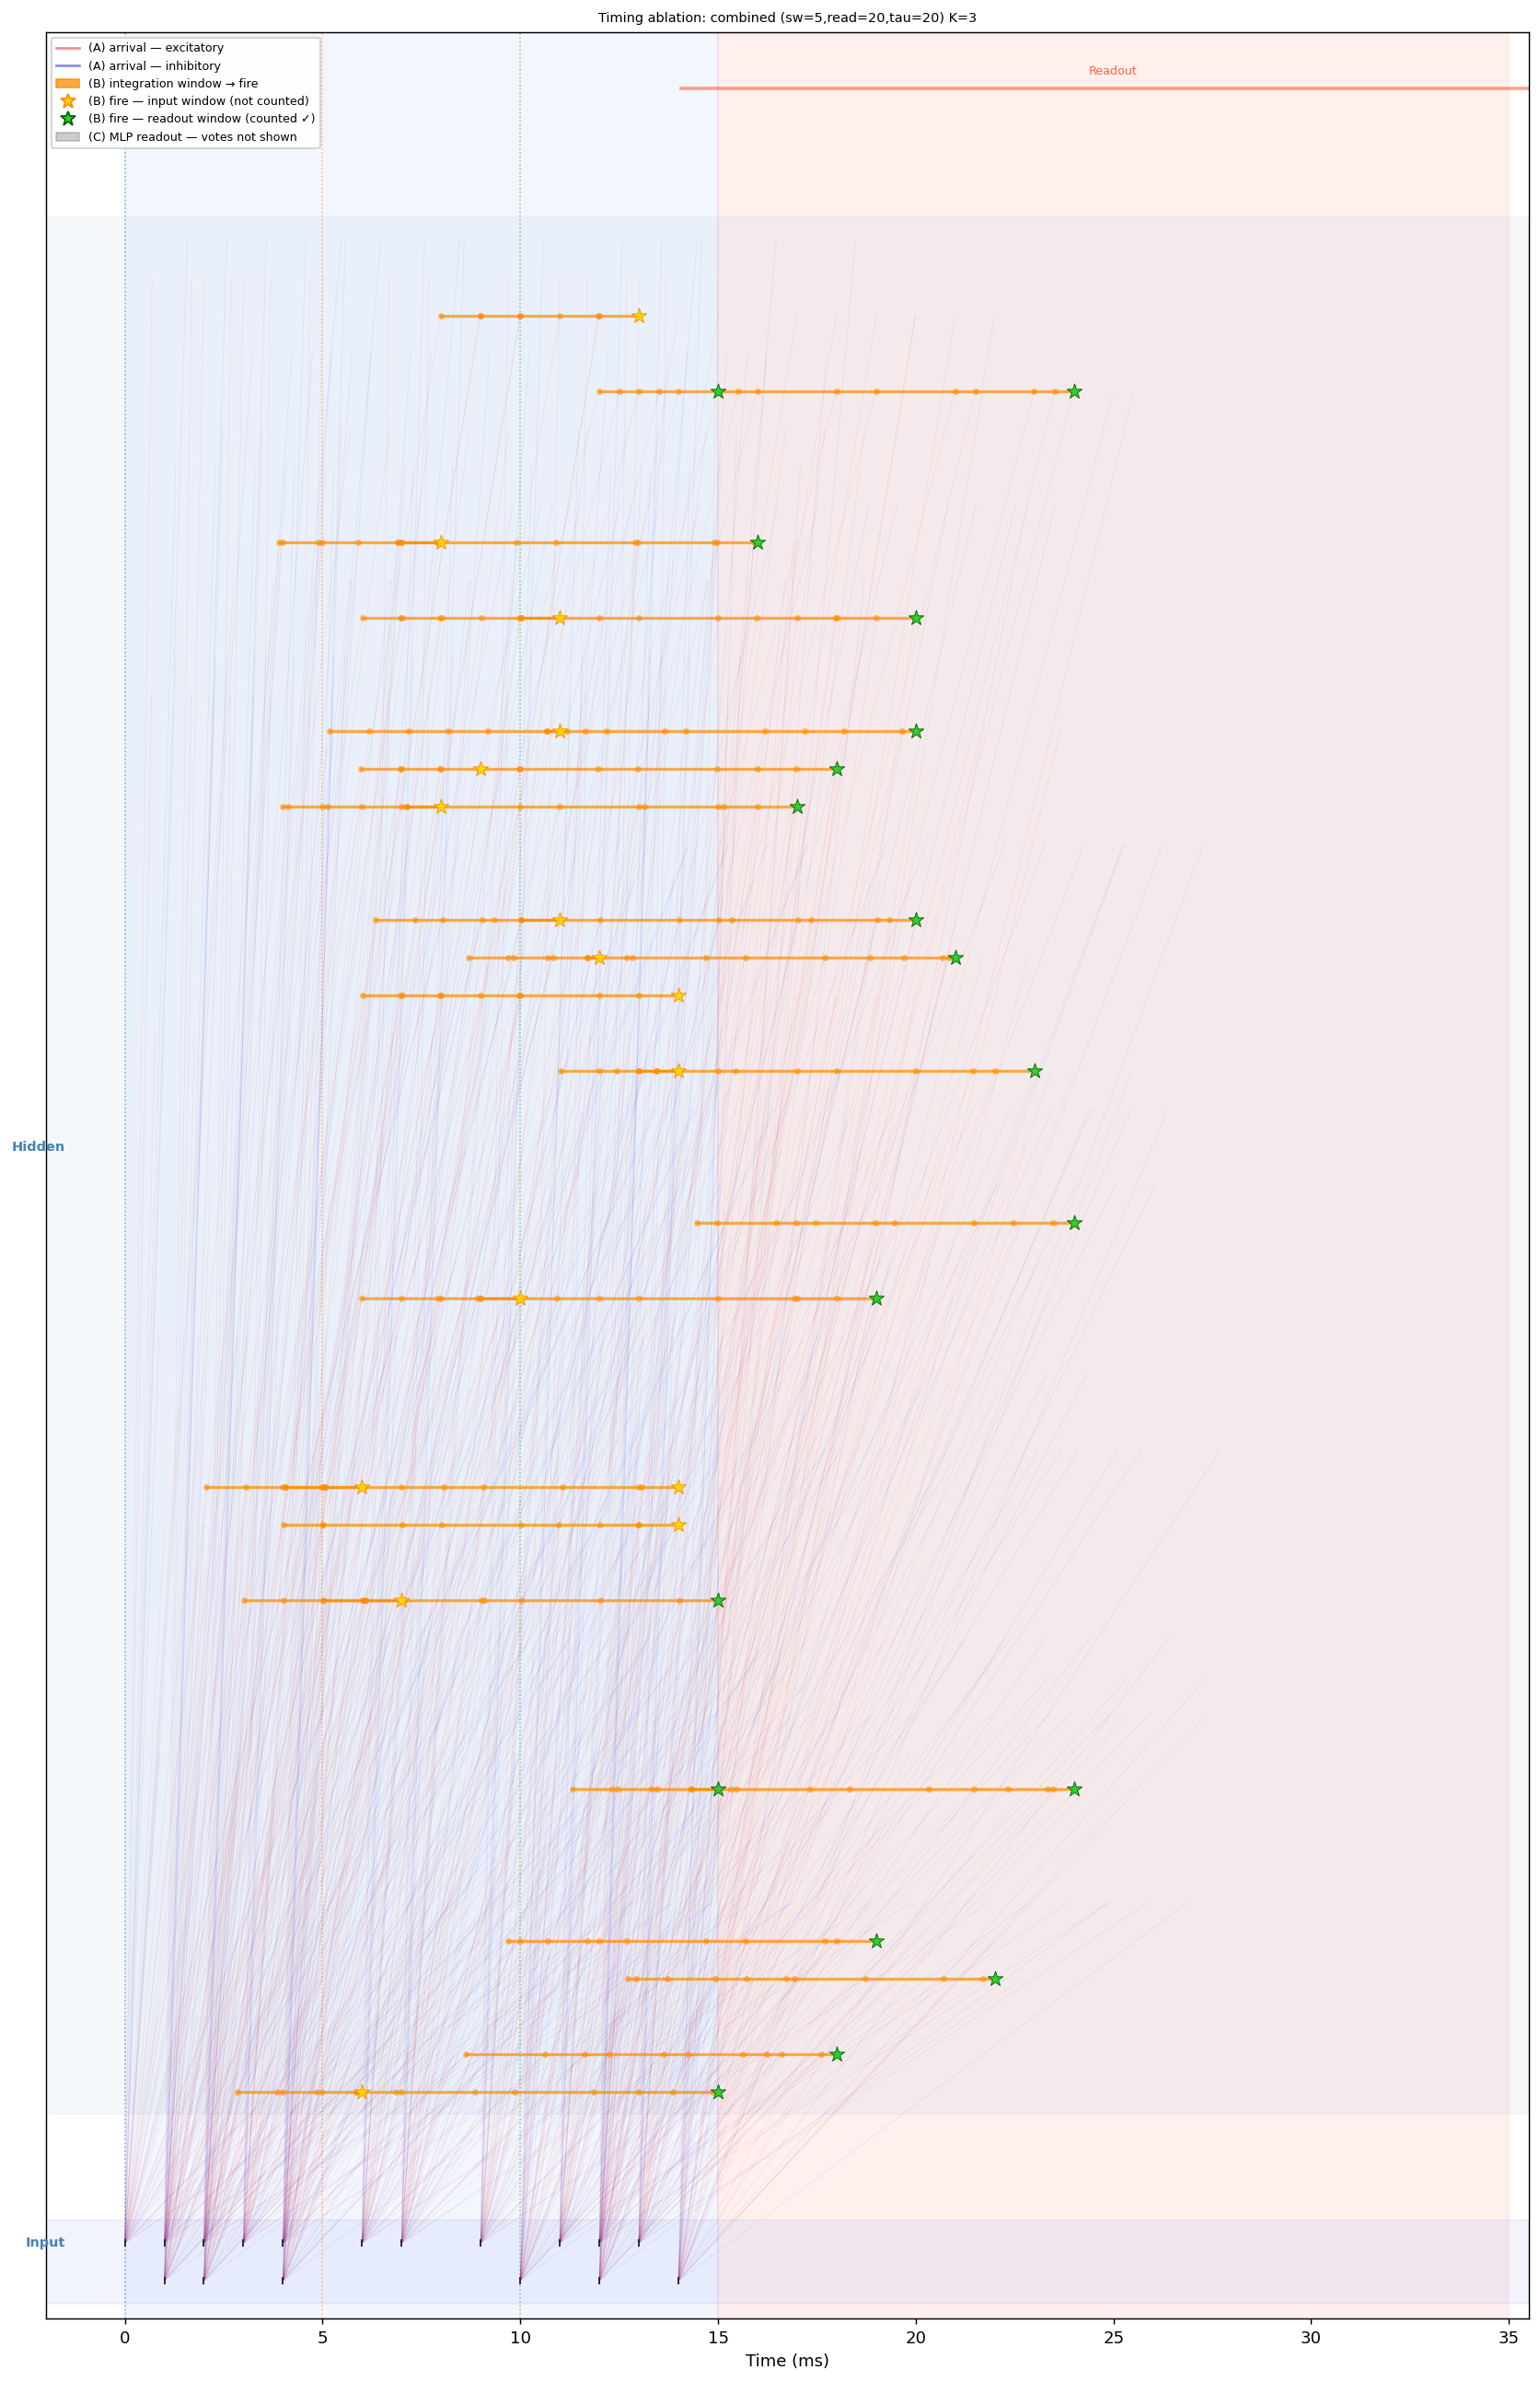
\includegraphics[width=0.31\textwidth]{timing_combined_K3_flow.png}
\caption{Enhanced spike flow, $K{=}3$, L1-h50+MLP+delay, left to right:
\texttt{baseline} (92.7\%), \texttt{tau20} (88.6\%), \texttt{combined} (82.6\%).
Raising $\tau_m$ visibly shifts orange integration spans and hidden fires earlier
(into the Q1 sub-window rather than just before the readout window), leaving fewer
green (readout-window) stars relative to gold (input-window) stars than baseline.}
\label{fig:timingflow}
\end{figure*}

\subsection{Capacity scaling: is it neuron count?}
A hidden-size sweep ($h\in\{10,20,30,50\}$, $K\in\{1,...,5\}$, SC design, MLP readout,
$\tau{=}90\%$) directly tests whether more neurons can buy a higher $K$, by finding the
minimum $h$ needed to reach 90\% accuracy at each $K$. $K{=}1$ and $K{=}2$ both need only
$h{=}10$, but $K{=}3$ requires jumping to $h{=}50$, and $K{=}4,5$ \emph{never} reach 90\%
at any tested $h\leq50$ (best: 89.8\% at $K{=}4$, 86.3\% at $K{=}5$, both with $h{=}50$).
The $d{=}0$ control never reaches 90\% at any $h\in\{10,20,30,50\}$ (max 84.9\%),
confirming the ceiling is about \emph{delay-enabled routing capacity}, not raw neuron
budget.

This neuron-count sweep answers "how many neurons does $K$ cost"; the complementary
question is "how much energy does $K$ cost" at a \emph{fixed} neuron budget.
Fig.~\ref{fig:energy} takes the $h{=}50$, MLP-readout, \texttt{weights\_and\_delays} run
from Section~\ref{sec:ablation} (95.9/93.5/92.7/89.8\% at $K{=}1$--$4$) and plots, on the
$y$-axis, the number of independent computations $K$ reliably answered per trial against,
on the $x$-axis, the energy that costs -- measured as total hidden spikes per trial, our
hardware-realistic proxy for compute budget (Section~\ref{sec:step1}'s
energy-normalised-throughput metric). The async (blue) series is \emph{measured}: real
spike counts from the actual multi-$K$ SC-design runs. The sync (grey) series is
\emph{not} measured the same way -- it is the analytic cost of $K$ \emph{independent}
single-query trials at the single-operation baseline's spike cost ($\sim$34
spikes/query), i.e.\ $E_{\text{sync}}(K)=K\times34.1$. This is not an unfair comparison: a
sync trial's accuracy is, by construction, independent of $K$ (the $K$ trials do not
share any resource, so one trial's outcome cannot interfere with another's), so the sync
series trivially clears the 90\% threshold at every $K$ -- the threshold is doing real
filtering work only on the async series, where shared-resource interference is exactly
the effect under study. Because the SC design shares one hidden layer and one readout
window across all $K$ queries, its spike cost grows far slower than linearly in $K$ (8
$\to$ 19 $\to$ 28 $\to$ 41 spikes for $K{=}1$--$4$), yielding a consistent
\textbf{73\% energy reduction} for the same number of computations at $K{=}2$ and
$K{=}3$ -- the same delay-enabled routing capacity described above, viewed through the
energy-normalised-throughput lens rather than the neuron-count lens. We scope this claim
explicitly to $K\!\leq\!3$, where \emph{both} series clear 90\%: at $K{=}4,5$ the async
series itself falls below threshold (the same capacity ceiling characterised above, not
an energy phenomenon), so we mark those points with $\times$ rather than either omitting
them or lowering $\tau$ to make them appear to clear it -- doing the latter would make
this figure inconsistent with the $\tau{=}90\%/95\%$ convention used everywhere else in
the paper.

\begin{figure*}[t]
\centering
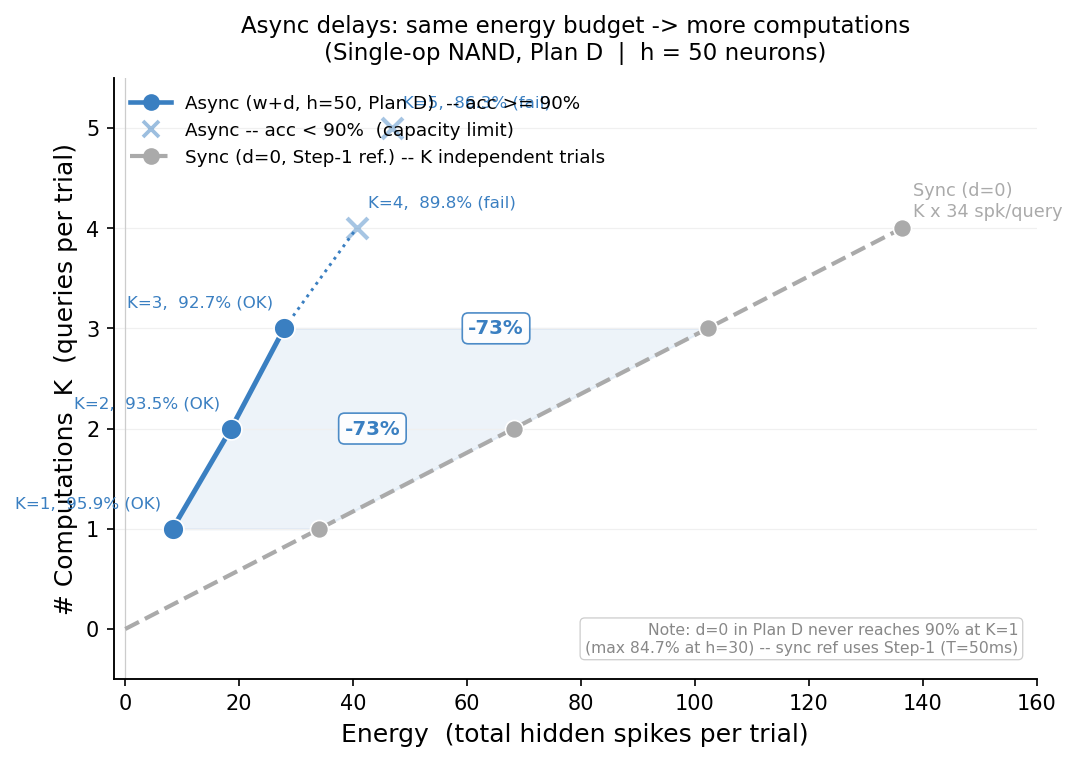
\includegraphics[width=0.6\textwidth]{fig_computation_energy.png}
\caption{Energy cost of $K$ computations at a fixed $h{=}50$ budget (NAND, SC design, MLP
readout, \texttt{weights\_and\_delays}). Async (blue, measured): $K$ queries multiplexed
in one trial. Sync (grey, analytic): $K$ independent single-query trials at the
single-operation baseline's spike cost -- accuracy is $K$-invariant by construction, so
this series always clears the 90\% line. The two crossed async points at $K{=}4,5$ fall
below the 90\% threshold (the same delay-enabled-capacity ceiling characterised by the
neuron-count sweep above); the 73\% energy-reduction claim is scoped to $K\!\leq\!3$,
where both series are at or above threshold.}
\label{fig:energy}
\end{figure*}

\section{Discussion: Is Max K@90\%$=$3 a Reasonable Ceiling?}
\label{sec:discussion}

A capacity ceiling near $K{=}3$ for a 50-neuron hidden layer is consistent with several
independent lines of prior work, suggesting it is not an artefact of our specific
implementation. The theta--gamma working-memory model posits $\sim$7$\pm$2 (later revised
to 4$\pm$1 \cite{cowan2001magical}) items multiplexed per oscillatory cycle in networks
with $\sim$10$^4$ neurons \cite{lisman1995storage}; polychronous-group analysis of
delay-coupled networks finds $\sim$20--50 groups per 1000 neurons
\cite{izhikevich2006polychronization}, which scales (very roughly, linearly) to
$\sim$1--2.5 at $h{=}50$ -- matching our linear-readout ceiling of $K{=}2$ and falling
just short of our MLP ceiling of $K{=}3$. The gap between \emph{learnable} and
\emph{theoretical} capacity that we observe (delay-structured representations exist that
a linear decoder cannot exploit, Section \ref{sec:2x2}) also mirrors the classical
result in associative memory that the practically learnable capacity of a Hopfield
network ($\sim$0.05$N$) falls well short of its information-theoretic capacity
($\sim$0.138$N$, \cite{hopfield1982neural,amit1985storing}). We read this as evidence that
the $K{=}3$ ceiling reflects a genuine representational-interference limit on how many
simultaneously-active temporal codes a shared population can keep linearly (or even
shallowly-nonlinearly) separable -- not a defect of our specific architecture, training
procedure, or timing constants (Section \ref{sec:ablation} rules out the latter
directly).

\section{Mixed-Operation Generalisation}
\label{sec:step3}

Sections \ref{sec:step2}--\ref{sec:ablation} use a single fixed operation (NAND) across
all $K$ queries in a trial. This section asks whether the same mechanism survives when each of
the $K$ queries in a trial uses a \emph{different} boolean operation (one-hot
op-identity channels are added to the input), on the best-known architecture from Section
\ref{sec:ablation} (L1+MLP+trainable delays).

\subsection{8 operations, then 4 operations: a data-sparsity wall}
With all 8 operations sampled uniformly ($n_{\text{train}}{=}4000$, $\sim$500/op), the
delay advantage generalises in magnitude (+11--20\% over $d{=}0$, matching single-op Plan
D) but \emph{absolute} accuracy is low: Max K@90\%$=0$ for both conditions, because
$\sim$500 samples/op is far below the $\sim$4000 samples that single-op NAND used.
Restricting to the 4 linearly-separable operations (AND/OR/NAND/NOR, removing
XOR/XNOR, $n_{\text{train}}{=}4000$, $\sim$1000/op) raises $K{=}1$ to 87.7\% but still
falls 2.3 points short of 90\% -- multi-function representational competition is an
\emph{independent} bottleneck from data sparsity.

\subsection{Direction A: matching single-op data density}
Increasing to $n_{\text{train}}{=}16000$ ($\sim$4000/op, matching single-op NAND's
density) confirms the data-sparsity hypothesis: $K{=}1$ jumps to 96.5\%, and
\textbf{Max K@90\% rises from 0 to 2}.

\subsection{Direction C: matching single-op capacity}
Doubling hidden size ($h{:}50\to100$, single layer, same 16k data) pushes $K{=}3$
from 88.1\% to 90.2\%, crossing the threshold: \textbf{Max K@90\% rises from 2 to 3},
\emph{exactly matching the single-operation ceiling} from Section \ref{sec:ablation}.

\subsection{Direction D: depth hurts here too}
Splitting the same 100-neuron budget into two layers ($h_1{=}50,h_2{=}50$) drops
Max K@90\% back down to 2 -- the same width-beats-depth pattern observed for single-op
NAND in Section \ref{sec:ablation}.

\begin{table}[t]
\centering
\caption{Mixed-operation progression, accuracy (mean of 2 seeds) and Max K@90\%.}
\label{tab:step3}
\begin{tabular}{lcccc}
\toprule
Variant & $K{=}1$ & $K{=}2$ & $K{=}3$ & Max K@90\% \\
\midrule
8op, $n{=}4$k & 84.3\% & 74.4\% & 68.7\% & 0 \\
4op, $n{=}4$k & 87.7\% & 80.2\% & 74.9\% & 0 \\
4op, $n{=}16$k (A) & 96.5\% & 93.0\% & 88.1\% & 2 \\
4op, $n{=}16$k, $h{=}100$ (C) & 97.0\% & 94.2\% & \textbf{90.2\%} & \textbf{3} \\
4op, $n{=}16$k, $h{=}50{+}50$ (D) & 94.75\% & 92.08\% & 88.72\% & 2 \\
\bottomrule
\end{tabular}
\end{table}

Fig.~\ref{fig:step3raster} shows the \texttt{weights\_and\_delays} rasters for Direction A
at $K{=}1,2,3$: as $K$ grows, the network maintains a clear query-staggered delay
structure (visible diagonal banding of spike times across Q0/Q1/Q2) -- the same
qualitative signature as the single-operation case (Section \ref{sec:pland},
Fig.~\ref{fig:k1}/\ref{fig:k2}, where the $d{=}0$ comparison is shown directly), now
reproduced under operation heterogeneity. The $d{=}0$ control is essentially insensitive
to both data volume and hidden size across all four mixed-operation variants (Table
\ref{tab:step3} omits this for space; it stays in the 53--70\% range throughout),
confirming delays -- not data or capacity alone -- are what convert available capacity
into temporal-multiplexing capability.

\begin{figure*}[t]
\centering
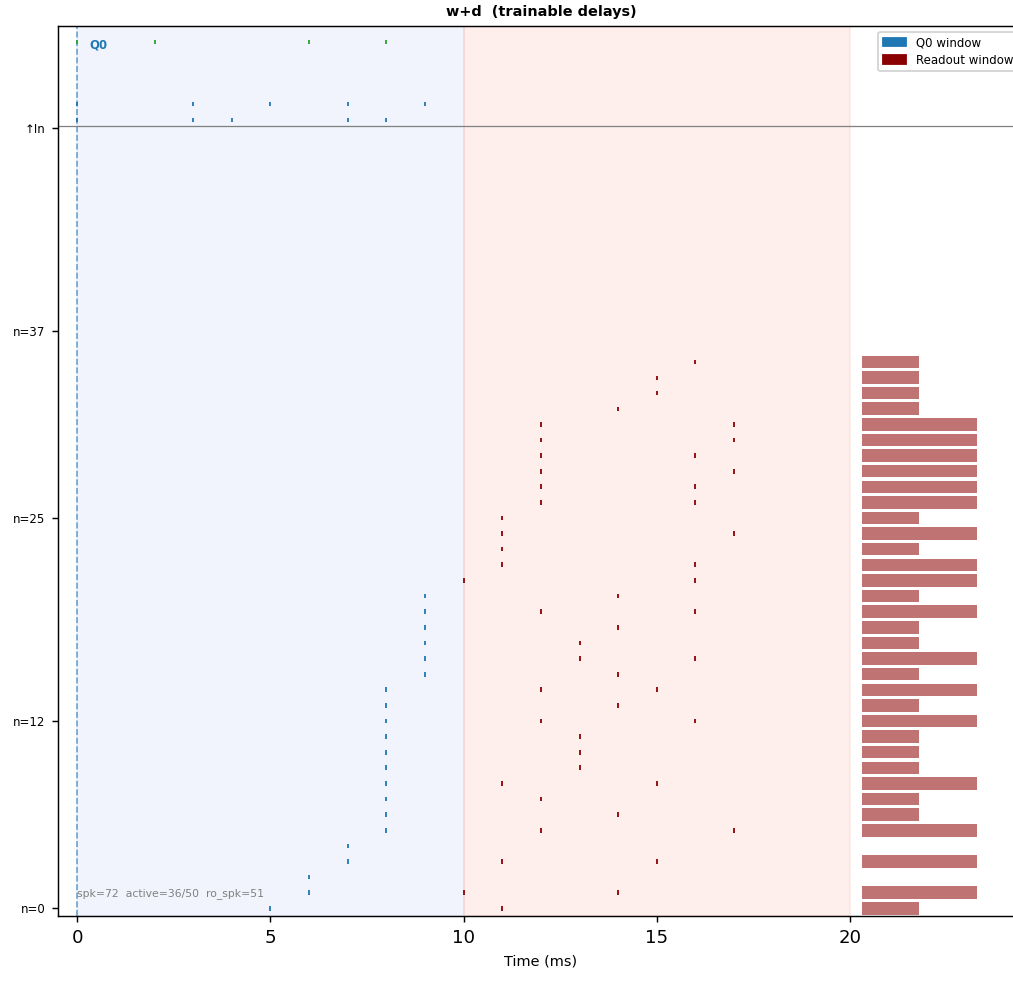
\includegraphics[width=0.31\textwidth]{fig_step3_k1_wad_only.png}\hfill
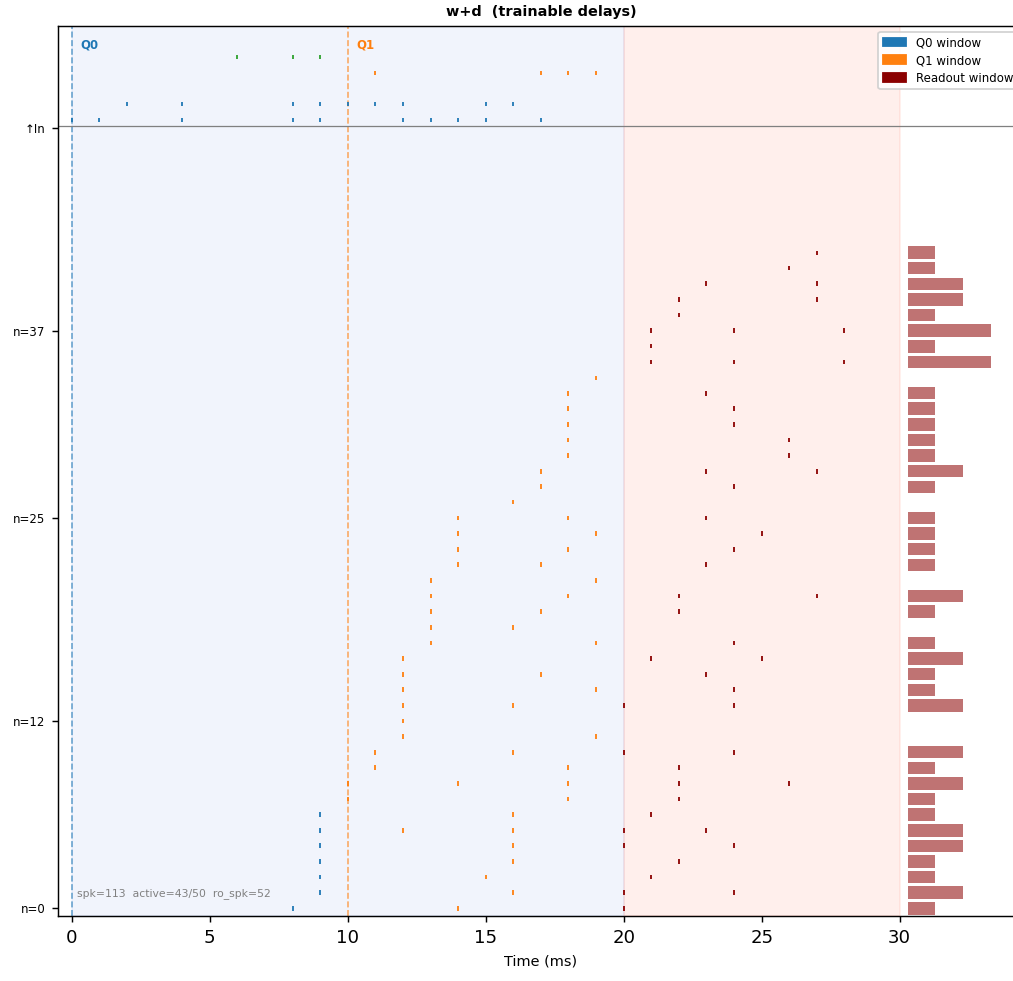
\includegraphics[width=0.31\textwidth]{fig_step3_k2_wad_only.png}\hfill
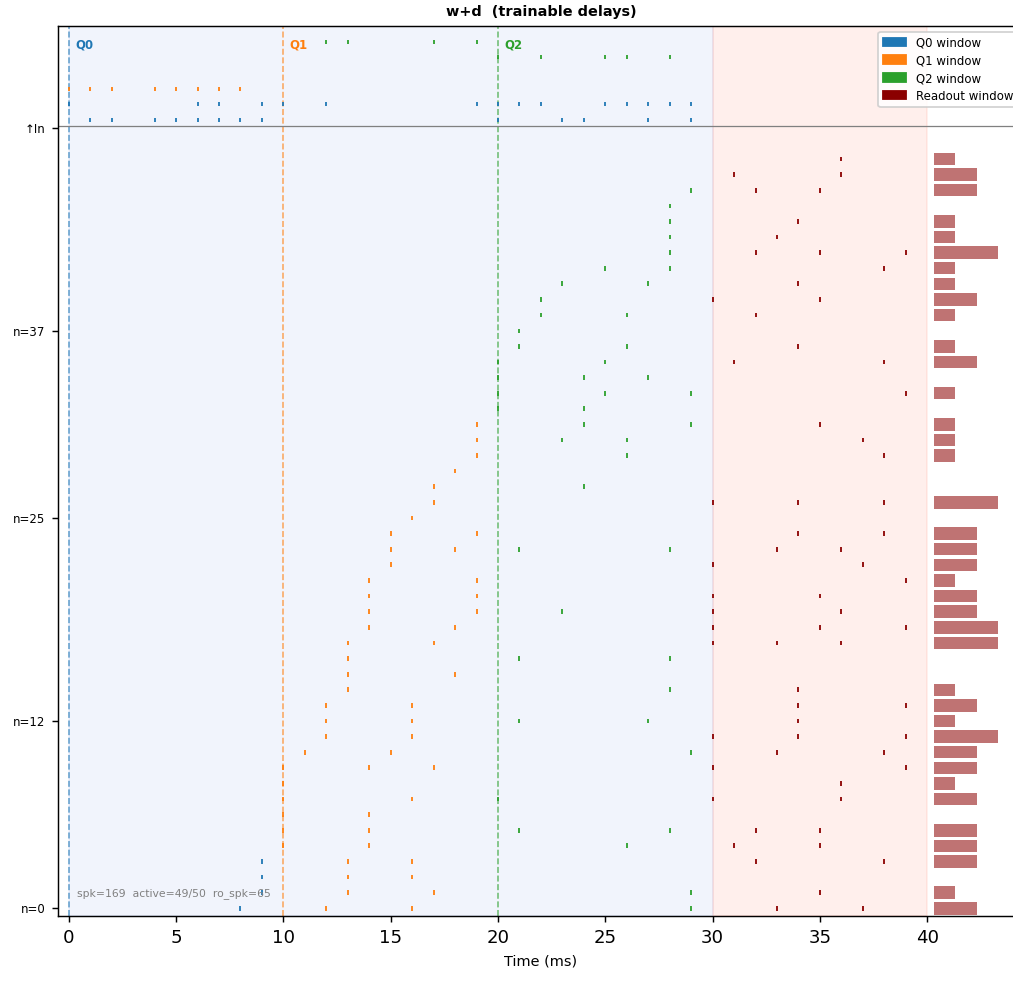
\includegraphics[width=0.31\textwidth]{fig_step3_k3_wad_only.png}
\caption{Mixed-op (4-op, $n{=}16$k, $h{=}50$, MLP), \texttt{weights\_and\_delays} rasters,
left to right $K{=}1,2,3$ (each panel cropped to the wad condition only, for legibility at
this width; the $d{=}0$ contrast for this task follows the same pattern already shown for
single-operation NAND in Fig.~\ref{fig:k1}/\ref{fig:k2}).}
\label{fig:step3raster}
\end{figure*}

\textbf{Overall:} once data volume and hidden-layer capacity are matched to the
single-operation case, mixed-operation trials reproduce the \emph{same} mechanism
(delay-driven query separation) and the \emph{same} capacity ceiling
(Max K@90\%$=$3) as single-operation NAND -- strong evidence that the core finding is
not an artefact of using a single fixed boolean function.

\section{Limitations and Future Work}
\label{sec:future}

This section lists, with the same level of concreteness as the completed experiments
above, exactly what remains before this work would be ready for a full conference
submission rather than an internal progress report.

\subsection{Untested input/output topologies}
All experiments above share one structure: $K$ \emph{different} queries map to $K$
\emph{different} outputs (``many-query, many-out''). Three structurally distinct
topologies, flagged in our experiment registry as planned but not started, would test
whether the same delay-routing mechanism generalises to other multiplexing patterns:
\begin{itemize}
\item \textbf{One-query, many-op} ($1\times(A,B)\to K$ different op outputs): a single
input pair is broadcast and the network must compute $K$ \emph{different} functions of
it simultaneously. This inverts the current setup (shared computation, divergent inputs
$\to$ divergent computation, shared input) and would test whether delay-based routing
can fan a single signal out to $K$ independent computational branches. Proposed design:
reuse the SC-design architecture but replace the $K$ sequential input sub-windows with a
single input window and $K$ parallel readout heads, each trained on a different boolean
function.
\item \textbf{Many-query, one-out} ($K$ same-op queries $\to$ 1 aggregate output, e.g.\
majority vote or AND-of-results): tests temporal \emph{integration} rather than
separation. Proposed design: keep the SC design's sequential-injection structure but replace
the $K$-logit readout with a single-logit readout trained on an aggregate label.
\item \textbf{Many-query, many-op, one-out}: the combination of the above -- $K$
heterogeneous queries aggregated to a single decision. Natural next step once the first
two are characterised.
\end{itemize}

\subsection{Isolating depth from neuron count}
Section \ref{sec:ablation}'s unconstrained-depth follow-up (L2-h50h50, 100 neurons,
$\text{readout\_in}{=}50$) reaches Max K@90\%$=$4 on single-operation NAND, better than
any single-layer configuration tested -- but we lack a single-layer $h{=}100$ control for
this task to confirm whether the gain comes from \emph{depth} or simply from
\emph{doubling the neuron count}. Running L1-h100-linear/MLP on single-operation NAND
(the same architecture already used for the mixed-operation task in
Section~\ref{sec:step3}, just retargeted) would directly settle this.

\subsection{Energy-matched accuracy comparison}
Our throughput metric ($K/\text{spikes}$) compares energy at whatever accuracy each
condition happens to reach. A more rigorous comparison would fix accuracy at $\tau{=}90\%$
and compare \emph{total spikes} between \texttt{weights\_and\_delays} and $d{=}0$ at each
condition's own minimum-$h$ configuration -- this is not yet measured and would more
directly support an ``energy efficiency'' claim.

\subsection{Quantifying temporal neuron reuse and inhibitory routing}
Visual inspection (Section \ref{sec:pland}, \ref{sec:ablation}) shows individual hidden
neurons participating in multiple queries via differentiated delays on their incoming
synapses (``temporal reuse''), and inhibitory connections appearing only once $K$
approaches the capacity boundary. Neither observation has been turned into a number:
proposed measurements are (i) the fraction of hidden neurons that fire in $\geq2$ distinct
query sub-windows at a given $K$, and (ii) the ratio of inhibitory to excitatory
propagation lines as a function of $K$, both extractable from the existing
\texttt{diagnostic\_data.npz} traces without retraining.

\subsection{A non-SNN baseline}
We have not compared against a non-spiking sequence model (e.g.\ an LSTM or a small MLP
reading the raw $[T,2]$ binned-spike tensor) on the SC-design task. This is the single
biggest gap if targeting a machine-learning venue rather than a neuromorphic-systems
venue: if a generic RNN matches our Max K@90\%$=$3 with comparable or fewer parameters,
the claim narrows to ``SNNs are one way to implement temporal routing'' rather than
``delays are a necessary mechanism for it.''

\subsection{Theoretical account of the linear/nonlinear decodability gap}
Section \ref{sec:ablation} shows empirically that delay-structured hidden representations
become linearly inseparable somewhere between $K{=}2$ and $K{=}3$. We do not yet have a
theoretical account of \emph{why} -- a natural starting point would be a
linear-separability or Rademacher-complexity argument over the geometry of $K$
superimposed, exponentially-decaying membrane traces (cross-slot residual
$e^{-\text{sw}/\tau_m}\approx37\%$ at our settings), which would let the $K{=}2/3$
boundary be predicted rather than only measured.

\subsection{Spiking readout layer}
We additionally tried replacing the linear/MLP readout with a third spiking (LIF) layer,
trained with \texttt{BCEWithLogitsLoss} on output spike counts. This trains slowly (a
dead-neuron problem for the first $\sim$90 epochs) and after 1000 epochs reaches only
71.8\% (vs.\ 43.6\% for $d{=}0$, a +28\% gap consistent with the rest of this paper) --
far below the 92.7\% a linear/MLP readout achieves at the same $K$. We do not consider
this a practical readout, but it remains useful for fully-spiking
input$\to$hidden$\to$output visualisation and is left as a training-method open problem
rather than pursued further here.

\subsection{Discrete (hardware-realistic) delays}
All delays above are continuous (sigmoid-parameterised, optionally rounded via a
straight-through estimator at inference). A discretised, hardware-realistic delay line
(fixed integer steps, quantisation-aware training) was deprioritised but would matter for
any claim about neuromorphic hardware implementability.

\section{Conclusion}

Using a minimal boolean-logic SNN testbed, we showed that trainable synaptic delays are
\emph{structurally} necessary -- not merely helpful -- for temporal multiplexing on
shared input channels: a delay-free network plateaus near a label-prior baseline
regardless of readout expressiveness (Section \ref{sec:ablation}). Across three
progressively constrained experimental designs, the dominant contribution of delays is
\emph{temporal alignment} (shifting signals into the readout window), four to five times
larger than the additional \emph{routing capacity} they provide; that capacity is real,
however, and is bounded by decoder expressiveness rather than raw neuron count, raising
Max K@90\% from 2 (linear readout) to 3 (one-hidden-layer MLP, at $h{=}50$). This same
mechanism and the same numerical ceiling reproduce under mixed-operation trials once
data volume and capacity are matched to the single-operation case. A literature-grounded
comparison (theta--gamma multiplexing, polychronization, associative-memory capacity
gaps) suggests $K{\approx}3$ for $h{=}50$ is a plausible, non-arbitrary order of
magnitude rather than an artefact of this implementation. Section \ref{sec:future} lists
the concrete experiments -- untested multiplexing topologies, an energy-matched
comparison, a non-SNN baseline, and a theoretical decodability account -- needed to move
from this internal progress report to a submission-ready paper.

\bibliographystyle{ieeetr}
\bibliography{refs}

\end{document}
